\newcommand{\aref}[1]{\autoref{#1}\space}
\newcommand{\eref}[1]{式\eqref{#1}}
\renewcommand{\algorithmcfname}{算法}
\chapter{绪论}
\section{研究背景与意义}
机器人一直是人类孜孜不倦探索钻研的目标,人类一直致力于实现让机器人覆盖人
类的功能,使人类从繁杂重复的体力劳动中或是危险系数较高的工作中解放出来。
陆地上移动的机器人主要分为轮履式机器人、躯干式机器人和腿足机器人。
就当今已存在的机器人中,轮式机器人和履带式机器人要占据绝大部分。这种类型机器人有着移动快,控制简
单,实现方便的特点,同时在平坦以及硬质路面有着移动速度较快的特性。但是此类机
器人无法适应复杂路面,比如轮式机器人无法实现在阶梯或是崎岖路面前进,履带式机
器人也很难做到上下楼梯。相比较来说,腿足式机器人就能很好适应复杂路面,在崎岖
路面有着得天独厚的优势,从人类通过双腿可以适应自然界绝大部分的地貌环境就可以
看出来,足式机器人更适合于复杂的陆地环境\cite{Schraft2000ServiceR}。人类通过视觉信息选取离散的落脚点
以跨过不同的障碍物和适应不同的路面,腿足式机器人可以通过步态规划以及身体平衡
控制做到不平整路面的行走,但目前仍然存在许多挑战。

目前国内外关于腿足式尤其是仿人机器人的研究也受到越来越多的关注,仿人机器
人是仿生机器人领域的代表之一,它集机械、电气、计算机、传感器等多种学科于一体,
是直接模仿采用仿人前进动物的一类机器人\cite{梶田秀司2007仿人机器人}。
腿足式也是自然界大部分生物所采取的运动方式,所以机器人采用腿足
式方式能够更好的融入人类生活中。采用和人类相似的外形使得腿足式机器人相对于轮
式和履带式机器人在亲和力方面有着难以匹敌的优势,完美的适应人类的工作环境\cite{2010067776.nh}。
在未来利用仿人机器人取代人类在高危险环境下的工作或者重复性较高的体力劳动的
是必然趋势。此外对于腿足式机器人的研究还能够通过得到腿部运动的规律设计康复外
骨骼等助力工具帮助残疾人恢复健康。对于腿足式机器人的研究能够更好的了解人类腿
部运动机理,利用康复性外骨骼机器人帮助腿部残疾的患者恢复健康也是大势所趋。

2011年日本发生福岛核泄漏事件,给当地人民的安全生活带来了很大隐患,
这使得人们开始考虑能否用仿人机器人代替维修工人进入这种高危环境中,
以尽可能地减少灾难环境下的生命财产损失。美国国防高级研究计划局(Defense Advanced Research Projects Agency,DRAPA)
从2012至2015年举办了DRC(DRAPA Robotics Challenge),旨在探索机器人在灾后的复杂环境中,代替人类执行任务的可能性。
DRC的任务中包括穿过废墟、驾驶车辆、爬上梯子、开门、关上阀门等等,极大地推进了仿人机器人的研究进展。
这些任务也十分明确地体现了仿人机器人特有的优势:对于复杂地形的适应,能够使用为人类设计的工具等。

仿人机器人存在结构复杂,自由度高,非线性强,本质不稳定等特点,其运动的性能、稳定性以及对复杂的人类环境的适应能力至今无法达到人们的期望。
但随着关节驱动技术、各种高效的优化求解库,以及机载计算平台算力的不断发展,仿人机器人的运动控制技术正逐渐趋于成熟。
虽然目前来看仿人机器人真正走向应用还需要很长时间,但开展针对仿人机器人运动控制的研究是很有必要的。
\section{国内外研究现状介绍}
\subsection{日本仿人机器人研究现状}
早在20世纪60年代末,日本就开始了对仿人仿人机器人的研究。
日本早稻田大学的Ichiro Kato教授于1969$\sim$1971年设计制作了液压驱动的
仿人机器人WL-3以及WL-5(\aref{subfig:wl5}),并以此为基础在1973年研制了仿人机器人WABOT-1 (\aref{subfig:wabot1}),
这也被认为是最早的现代仿人机器人。
尽管这些机器人运动能力相当差,
\begin{figure}[htbp]
    \centering
    \subcaptionbox{WL-5\label{subfig:wl5}}
        {%
            \includegraphics[height = .3\linewidth]{WL-5.jpg}}
    \subcaptionbox{WABOT-1\label{subfig:wabot1}}
        {%
            \includegraphics[height = .3\linewidth]{WABOT-1.jpg}}
    \caption{早稻田大学研制的早期仿人机器人\label{fig:japan_old}}
\end{figure}
只能实现一些静态动作,但也在客观上引发了学术界和产业界对仿人仿人机器人研究的兴趣。
\begin{figure}[htbp]
    \centering
    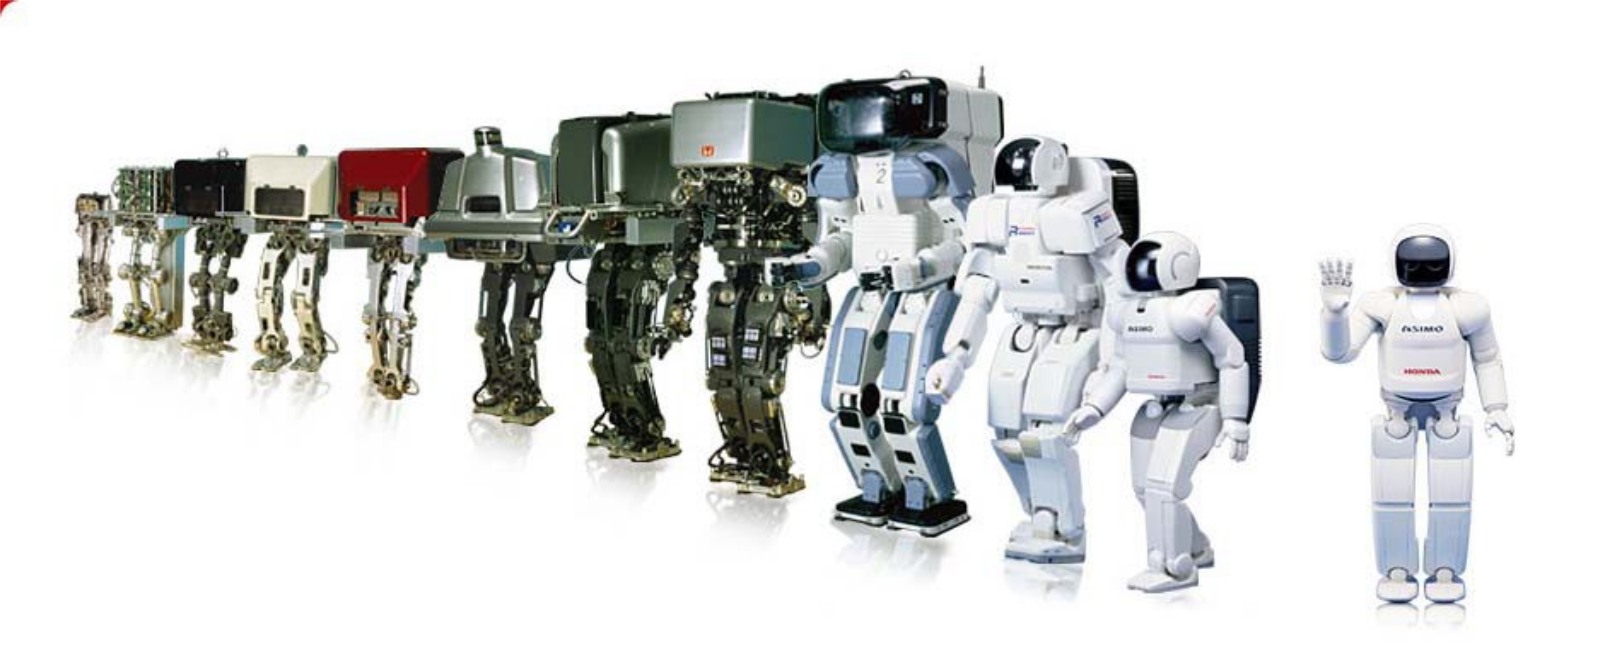
\includegraphics[width=.8\linewidth]{asimo.jpg}
    \caption{\label{fig:asimo}本田公司研制的ASIMO仿人机器人及其历代原型机}
\end{figure}

20世纪80年代,日本本田公司也开始了仿人机器人的研究,
出于控制方便和动力源可携带等方面的考虑,本田选择了电机驱动的技术路线,
经过E0到E6的七代步行样机研发,以及加入仿人上半身的P1到P2的原型机迭代,以及基于P系列原型机做出的小型化改进,终于在2000年推出了著名的
仿人机器人ASIMO(\aref{fig:asimo})。 ASIMO具有良好的外观设计,并且集成了视觉识别、语音交互等技术,是最为人所熟知的仿人机器人之一。
本田也不断地对ASIMO进行改进,到2011年时ASIMO的奔跑速度就达到了9km/h,并能完成上下台阶、倒水等展示任务\cite{Honda}。
\begin{figure}[htbp]
    \centering
    \subcaptionbox{HRP-1\label{subfig:HRP-1}}
        {%
            \includegraphics[height = .3\linewidth]{HRP-1.jpg}}
    \subcaptionbox{HRP-2\label{subfig:HRP-2}}
        {%
            \includegraphics[height = .3\linewidth]{HRP-2.jpg}}
    \subcaptionbox{HRP-3\label{subfig:HRP-3}}
        {%
            \includegraphics[height = .3\linewidth]{HRP-3.jpg}}

    \subcaptionbox{HRP3L-JSK\label{subfig:HRP3L-JSK}}
        {%
            \includegraphics[height = .3\linewidth]{HRP3L-JSK.jpg}}   
    \subcaptionbox{HRP-4c\label{subfig:HRP-4c}}
        {%
            \includegraphics[height = .3\linewidth]{HRP-4c.jpg}}       
    \subcaptionbox{HRP-4\label{subfig:HRP-4}}
        {%
            \includegraphics[height = .3\linewidth]{HRP-4.jpg}}       
    \subcaptionbox{HRP-5P\label{subfig:HRP-5P}}
        {%
            \includegraphics[height = .3\linewidth]{HRP-5P.jpg}}       

    \caption{HRP系列仿人机器人\label{fig:japan_hrp}}
\end{figure}

除ASIMO外,日本产业技术综合研究院也在1998年开启了仿人机器人项目(Humanoid Robotics Project, HRP),HRP系列(\aref{fig:japan_hrp})
也采取了电机位置伺服驱动的思路,2018年第五代最新的HRP-5P发布(\aref{subfig:HRP-5P})。HRP-5P高182cm,重101kg,搭载的视觉和激光传感器可以识别工具类别并灵活使用工具,
并且具备搬运木板等较重负载的能力\cite{HRP},体现了HRP系列仿人20多年的研究积累。
\begin{figure}[htbp]
    \centering
    \includegraphics[height=.3\textwidth]{s-one1.jpg}
    \includegraphics[height=.3\textwidth]{s-one2.jpg}
    \includegraphics[height=.3\textwidth]{s-one3.jpg}
    \caption{\label{fig:s-one}S-One机器人完成DRC的各项任务}
\end{figure}

在参与HRP计划的研究机构中,东京大学的情报工学研究室(Johou Systems Kougaku Laboratory,JSK)取得的成果较为突出,2010年,JSK的Urata和Nakanishi
创造性地给伺服电机加入液冷系统,大大提高了电机的散热效率,再加上他们设计的大电流驱动器,整套驱动系统的功率密度得到了显著提升。
他们将改造过的驱动系统安装在了一对源于HRP-3的腿上从而得到了HRP3L-JSK(\aref{subfig:HRP3L-JSK}),HRP3L-JSK强大的驱动性能使其同时具有了快速运动和承受大负载的能力。
Urata等人之后创建SCHAFT公司,在HRP3L-JSK的基础上开发了S-One。搭载了强大驱动系统的S-One在DRC2013中成功完成了各项任务(\aref{fig:s-one}),以大比分优势取得了第一名,
SCHAFT也在2013年被Google收购。SCHAFT之后在2016年发布了其新研发的直线腿式仿人机器人,该机器人能够自主上下楼梯,并且能够在足底打滑的情况下快速恢复平衡\cite{SCHAFT}。
\subsection{美国仿人机器人研究现状}
从20世纪80年代开始,Marc Raibert及其领导的MIT腿机器人实验室(MIT LegLab)研发了一系列具备动态平衡及跳跃能力的腿足机器人。他们采取了由单腿到多腿,
由平面到三维的由简到繁递进的研究思路,利用压缩气体动力源高能量密度的优势,实现了即使放到今天也相当惊人的效果。1980至1982年他们研制了第一台跳跃机器人
Planar One-Leg Hopper(\aref{subfig:one-leg-2d}),该机器人由气缸驱动腿部的摆动和伸缩,可以实现平面约束下连续的稳定跳跃;在1983至1984年这个平面单腿机器人被拓展到了三维空间,
3D One-Leg Hopper(\aref{subfig:one-leg-3d})实现了在三维空间的连续稳定跳跃;1985至1990年间,Raibert又将平面单腿机器人拓展成为平面仿人机器人Planar Biped(\aref{subfig:biped-2d}),
实现了平面约束下的奔跑、越障、空翻等动作;后面Planar Biped 又进一步被拓展为3D Biped(\aref{subfig:biped-3d}),该仿人机器人能够在三维空间进行跑跳运动并完成空翻动作\cite{raibert1986legged}。
\begin{figure}[htbp]
    \centering
    \subcaptionbox{Planar One-Leg Hopper\label{subfig:one-leg-2d}}
        {%
            \includegraphics[height = .45\linewidth]{leglab1.jpg}}
    \subcaptionbox{3D One-Leg Hopper\label{subfig:one-leg-3d}}
        {%
            \includegraphics[height = .45\linewidth]{leglab2.jpg}}
    \caption{MIT LegLab 早期的单腿跳跃机器人\label{fig:leglab}}
\end{figure}

\begin{figure}[htbp]
    \centering
    \subcaptionbox{Planar Biped\label{subfig:biped-2d}}
        {%
            \includegraphics[height = .425\linewidth]{leglab3.jpg}}
    \subcaptionbox{3D Biped\label{subfig:biped-3d}}
        {%
            \includegraphics[height = .425\linewidth]{leglab4.jpg}}
    \caption{MIT LegLab 早期的仿人机器人\label{fig:leglab_biped}}
\end{figure}

此后Raibert离开MIT,创建了波士顿动力公司(Boston Dynamics)继续进行腿足机器人的相关研究。2009年,波士顿动力发布了新一代的仿人机器人PETMAN(\aref{fig:leglab_biped}),
PETMAN继承了MIT LegLab 时期的驱动思路,采用了同为流体驱动的液压驱动方案,它能模仿人的行走步态,并具有一定抗外界干扰的能力[8]。在PETMAN的基础上,
波士顿动力公司从2013年开始又进一步研发了Atlas,为其升级了动力系统,并增加了深度相机、激光雷达等传感器。Atlas被IHMC使用参加了DRC2015(\aref{fig:atlas})并取得了第二名。
\begin{figure}[htbp]
    \centering
    \subcaptionbox{PETMAN Prototype\label{subfig:biped-2d}}
        {%
            \includegraphics[height = .5\linewidth]{petman1.jpg}}
    \subcaptionbox{PETMAN\label{subfig:biped-3d}}
        {%
            \includegraphics[height = .5\linewidth]{petman2.jpg}}
    \caption{波士顿动力公司研发的两代PETMAN样机\label{fig:leglab_biped}}
\end{figure}
\begin{figure}[htbp]
    \centering
    \includegraphics[height=.36\linewidth]{atlas.jpg}
    \caption{\label{fig:atlas}IHMC参加DRC2015使用的Atlas机器人}
\end{figure}

随后波士顿动力公司将Atlas进一步小型化,为其开发了人机协作搬运货物等功能。小型化的Atlas能够自带电池在野外复杂环境行走,不再依赖于实验室的理想环境。从2018年开始,
波士顿动力公司每年都会发布Atlas的最新进展,采取液压驱动方案的Atlas也被公认为是世界上最先进的仿人仿人机器人。到2021年,Atlas已经能够完成后空翻、高难度跑酷、
甚至是跳舞等各种复杂高动态动作(\aref{fig:atlas_dance}),目前其他所有公开的仿人仿人机器人都无法在运动能力上望其项背。
\begin{figure}[htbp]
    \centering
    \includegraphics[height=.344\linewidth]{dance1.jpg}
    \includegraphics[height=.344\linewidth]{dance2.jpg}
    \includegraphics[height=.32\linewidth]{dance3.jpg}
    \includegraphics[height=.32\linewidth]{dance4.jpg}
    \caption{\label{fig:atlas_dance}Atlas机器人完成各种高难度动作}
\end{figure}

除Atlas外,美国的其他研究机构也在仿人机器人领域取得了瞩目的成就。密歇根大学的Jessy Grizzle教授在1997年开始研究平面仿人机器人,先后研发了RABBIT(\aref{subfig:RABBIT})
和MABEL(\aref{subfig:MABEL}),MABEL利用弹性机构储能,大大突破了电机功率密度的限制,可在平面约束下以1.95m/s进行奔跑,并且能够跨越障碍。在此基础上,Grizzle又和
俄勒冈州立大学的Jonathan Hurst教授合作研发了ATRIAS\cite{rezazadeh2015toward}(\aref{subfig:ATRIAS})以及MARLO\cite{buss2014preliminary}(\aref{subfig:MARLO})
两代3D仿人机器人,设计有板簧储能元件以及轻量化的腿部连杆,几乎所有的质量都集中在身体部位,能以最高9.1km/h的速度奔跑,并能应对台阶、室外斜坡等复杂路况。
\begin{figure}[htbp]
    \centering
    \subcaptionbox{RABBIT\label{subfig:RABBIT}}
        {%
            \includegraphics[height = .225\textheight]{michigan1.jpg}}
    \subcaptionbox{MABEL\label{subfig:MABEL}}
        {%
            \includegraphics[height = .225\textheight]{michigan2.png}}
    \subcaptionbox{ATRIAS\label{subfig:ATRIAS}}
        {%
            \includegraphics[height = .225\textheight]{michigan3.jpg}}
    \subcaptionbox{MARLO\label{subfig:MARLO}}
        {%
            \includegraphics[height = .225\textheight]{michigan4.jpg}}
    \caption{Jessy Grizzle和Jonathan Hurst合作研发的仿人机器人\label{fig:michigan_biped}}
\end{figure}

Jonathan Hurst在此前研究的基础上创办了Agility Robotics,而后者于2017年发布了仿人机器人Cassie\cite{Cassie}(\aref{subfig:Cassie})。Cassie由电机驱动,每条腿具备5个驱动自由度和
2个欠驱动自由度,能以2.1m/s的速度高速行走,并具备对户外复杂地形的良好适应能力。2019年Agility Robotics又发布了给cassie加入上身和双臂的仿人机器人Digit\cite{Digit}(\aref{subfig:Digit}),
Digit的设计目标在于和无人驾驶车队配合,解决无人配送最后的送货上门问题。
\begin{figure}[htbp]
    \centering
    \subcaptionbox{Cassie\label{subfig:Cassie}}
        {%
            \includegraphics[height = .4\linewidth]{cassie.jpg}}
    \hspace{1in}            
    \subcaptionbox{Digit\label{subfig:Digit}}
        {%
            \includegraphics[height = .4\linewidth]{digit.jpg}}
    \caption{Agility Robotics研发的两款仿人机器人产品\label{fig:michigan_biped}}
\end{figure}

\subsection{其他国家仿人机器人研究现状}
德国慕尼黑工业大学在2009年发布了仿人机器人Lola\cite{buschmann2009humanoid}。Lola多个关节采用了电机+滚珠丝杆的传动方式,尽可能减小腿部的转动惯量,可以以2.4km/h的速度步行。在2021年最新发布的视频中,
Lola以及可以应对不规则的路面,并可以在走过易打滑路面的时候利用双手支撑侧面墙壁以避免失稳\cite{Lola}(\aref{fig:lola})。
\begin{figure}[htbp]
    \centering
    \includegraphics[width=0.40\textwidth]{lola.jpg}
    \caption{\label{fig:lola}慕尼黑工大Lola机器人手臂辅助行走}
\end{figure}

意大利技术研究院(Italian Institute of Technology,IIT)在腿足机器人领域有着许多卓越的成果,2007年IIT推出了儿童尺寸的仿人机器人iCub\cite{tsagarakis2007icub}(\aref{subfig:iCub}),iCub装备了
具有触觉感知的人造皮肤等一系列传感器,但行走并不是它的主要设计目标,因此iCub的运动能力很差。除了iCub外,IIT在2012年公布了以行走功能为重点的COMAN\cite{dallali2012global}(\aref{subfig:COMAN}),
它的关节由SEA驱动,SEA带来的关节力控制效果使得COMAN在站立平衡恢复方面展现出优异的性能,但电机的功率限制决定了COMAN的行走性能非常一般。之后2013年IIT又参与了欧盟的
Whole-body Adaptive Locomotion and Manipulation项目,在随后的四年中研发了两款WALK-MAN机器人\cite{tsagarakis2017walk}(\aref{subfig:WALK-MAN}),但运动性能相比COMAN并未有显著的提升。

\begin{figure}[htbp]
    \centering
    \subcaptionbox{iCub\label{subfig:iCub}}
        {%
            \includegraphics[height = .4\linewidth]{iCub.jpg}}
    \subcaptionbox{COMAN\label{subfig:COMAN}}
        {%
            \includegraphics[height = .4\linewidth]{coman.jpg}}
    \subcaptionbox{WALK-MAN\label{subfig:WALK-MAN}}
        {%
            \includegraphics[height = .4\linewidth]{walkman.jpg}}            
    \caption{IIT的几款仿人机器人\label{fig:iit_biped}}
\end{figure}
\begin{figure}[htbp]
    \centering
    \includegraphics[height=.4\linewidth]{kaist1.jpg}
    \includegraphics[height=.4\linewidth]{kaist2.jpg}
    \includegraphics[height=.4\linewidth]{kaist3.jpg}
    \caption{\label{fig:kaist_hubo}KAIST-HUBO机器人及其多种运动形态}
\end{figure}

韩国先进技术研究院(Korea Advanced Institute of Science and Technology,KAIST)从2002年开始迭代研发了一系列KHR/HUBO仿人机器人,从2002年的KHR-1开始,
到2013年参加DRC的DRC-HUBO已经是第七代了。DRC-HUBO采用轮腿混合的设计,既能以仿人形态行走,也能跪下利用膝盖上的轮子移动\cite{zucker2015general}(\aref{fig:kaist_hubo})。
可以根据不同情境选择移动方式的优势使得DRC-HUBO最终夺得了DRC2015的冠军。
\subsection{我国仿人机器人研究现状}
\begin{figure}[htbp]
    \centering
    \subcaptionbox{先行者\label{subfig:poineer}}
        {%
            \includegraphics[height = .3\linewidth]{domestic1.jpg}}
    \subcaptionbox{汇童\label{subfig:sboy}}
        {%
            \includegraphics[height = .3\linewidth]{domestic2.jpg}}
    \subcaptionbox{KONG\label{subfig:KONG}}
        {%
            \includegraphics[height = .3\linewidth]{domestic4.png}}     
    
    \subcaptionbox{悟空-II\label{subfig:wukong2}}
        {%
            \includegraphics[height = .3\linewidth]{wukong2.jpg}}
    \subcaptionbox{悟空-III\label{subfig:wukong3}}
        {%
            \includegraphics[height = .3\linewidth]{wukong3.jpg}}            
    % \subcaptionbox{THBIP-I\label{subfig:THBIP-I}}
    %     {%
    %         \includegraphics[height = .4\linewidth]{domestic3.jpg}}         
    \caption{国内部分仿人机器人\label{fig:domes_biped}}
\end{figure}
早在1985年哈尔滨工业大学就研制了HIT-III仿人机器人,这也被认为是我国最早的仿人机器人\cite{谢涛2002}。该机器人由电机驱动,仅仅能够进行基本的静态步行。
国防科技大学1995年公布的KDW-III仿人机器人也仅能实现0.36km/h的静态步行。随后国防科技大学又在2001年公布了仿人机器人“先行者”(\aref{subfig:poineer}),是国内第一台具有可运动四肢的仿人机器人。
北京理工大学2000年开始了仿人机器人的研究,之后发布了“汇童”系列仿人机器人(\aref{subfig:sboy})。2006年发布的第二代汇童机器人已经具备了1km/h的动态行走能力,同时可以实现打太极、舞剑等全身动作。
第四代和第五代又分别实现了表情控制和打乒乓球的功能。目前最新的第六代汇童机器人可以实现倒地爬起、原地跳跃等功能\cite{huang2019historical}。浙江大学于2011年公布了仿人机器人KONG\cite{sun2011balance}(\aref{subfig:KONG})。
该机器人全身共计32个自由度,高160cm,重65kg,步行速度可达1.07km/h,能够实现和人对打乒乓球的功能。在2018年浙江大学又推出了可以实现跑跳步态的仿人机器人“悟空-II”,能以4km/h的速度跑步前进。2020年的“悟空-III"机器人完成了室外草地
行走实验,是国内率先实现室外草地行走的仿人机器人。
截至2022年,国内公开的仿人机器人中,更多还是借鉴了日本在仿人机器人领域的技术路线,采用高速电机加大速比减速器的关节驱动方案,运动性能基本还都局限在低速静态步行,
难以实现仿人机器人的动态步行及适应相对不平整的路面或台阶,相较国外还有相当大的差距。
\section{仿人机器人运动控制的典型方法}
目前仿人机器人运动控制最常用的方法主要有:基于ZMP的质心规划控制方法,基于简化模型的力控制方法,基于全身模型的力控制方法。
除此之外基于运动发散量(Divergent Component of Motion,DCM)的方法\cite{mesesan2019dynamic},基于捕获点(Capture Point)的方法\cite{koolen2012capturability},
以及基于混合零动力学(Hybrid Zero Dynamics,HZD)的方法\cite{hereid2019rapid}等也在仿人机器人运动控制领域内发挥着重要作用,
这里限于篇幅仅对上述三种具有代表性的典型方法作简要介绍。
\subsection{基于ZMP的质心规划控制方法}
ZMP(Zero Moment Point,零力矩点)最初由Vukobratovic等在1972年提出\cite{vukobratovic2004zero},Vukobratovic将其作为机器人稳定性的判据,指出当ZMP位于机器人支撑多边形内时,
机器人受到的合外力不会使其发生倾倒,从而说明机器人是稳定的,这一判据也被双足机器人界广泛接受,成为学界最为重要的双足稳定性判据之一。
Sardain等人提出了CoP(Center of Pressure,压力中心点)的概念,但后来的研究表明就衡量双足机器人行走稳定性而言,这两个指标是等价的。采用高转速小扭矩电机加大速比减速器关节驱动方案的双足机器人,由于传动链上摩擦等非线性因素太多导致难以做到关节实时力控制,
同时高减速比带来的不可后驱性又导致关节柔顺性很差,这些结构性问题导致这类机器人内生性地选择了关节位置控制,而ZMP的概念又为其方便地提供了规划质心轨迹的依据,
二者相辅相成,自然地形成了基于ZMP的位置控制技术路线。

当机器人在平地上运动时,足端所有接触点都是共面的,足底接触力通常可以等效到到足底的ZMP处,而ZMP在接触点组成的凸包内\cite{wieber2002stability}
(通过单向接触约束的多面体投影,非平面的接触点也有类似的性质\cite{caron2016zmp})。在这种情况下,预先定义好质心在竖直方向上的运动可以得到高效的线性模型。其中最常见的是线性倒立摆模型(Linear Inverted Pendulum,LIP),
它假设质心在平面内运动并且角动量为0\cite{kajita1991study}。考虑非零的角动量并不影响模型的线性,但很少有人这样做,
主要是在平地上行走时这样做的好处并不多\cite{koolen2012capturability}。ASIMO是采用ZMP方法进行机器人行走控制的代表,前文提到的国内北京理工大学汇童系列机器人和浙江大学KONG机器人也均采用了这种规划质心轨迹的方法。

ZMP类的方法基于位置控制,在平地上能起到较好的控制效果,然而一旦路面变得不平整机器人就很难获得实际ZMP点的位置,从而导致控制器规划出的质心轨迹无法使机器人保持稳定。
并且在受到外力干扰时,控制器也很难快速做出响应,往往导致机器人失稳。抗干扰能力的缺失限制了基于ZMP的控制方法,也限制了采用这类控制方法的仿人机器人的应用场景。

\subsection{基于简化模型的力控制方法}
关节力控制作为一个较为通用的控制方法,在操作臂领域很早就得到了较为广泛的运用,通过控制关节空间的力矩,可使机器人在操作空间表现出不同的力特性。
基于力控制的方法,不再追求规划仿人机器人各关节的轨迹,而是直接对机器人关节力矩做控制,使机器人在笛卡尔空间保持平衡,并执行期望的运动。
力控制方法赋予了仿人机器人对复杂环境的适应能力,同时也能对外力扰动做出比较迅速的响应。

仿人机器人的简化模型通常是质心模型的某种变形。基于简化模型的力控制方法更加关注和地面接触力直接绑定的质心动力学,而不是和关节力矩直接绑定的
机器人的精准全身动力学\cite{vukobratovic1972contribution},如\aref{fig:centroid}所示。弹簧倒立摆(Spring Loaded Invert Pendulum, SLIP)模型是仿人机器人
运动控制中最常用的简化模型之一,MIT的Marc Raibert早在20世纪80年代就对SLIP模型进行了系统的阐述\cite{raibert1986legged}。他基于SLIP模型的三通道解耦控制理论
在MIT LegLab的单腿跳跃机器人3D One-Leg Hopper以及双腿跳跃机器人3D Biped上均得到了验证。

\begin{figure}[htbp]
    \centering
    \includegraphics[width=.5\linewidth]{质心动力学.eps}
    \caption{\label{fig:centroid}质心动力学及其与全身动力学的联系释图(图源\cite{carpentier2016center})}
\end{figure}
基于简化模型的力控制方法不要求对仿人机器人进行准确的动力学建模,因而比较容易在实际机器人上得到验证并取得的良好效果。但在受高阶动力学因素影响较大的运动场景中
简化模型的局限性就会体现出来,比如高速奔跑、跳跃等场景。
\subsection{基于全身模型的力控制方法}
新的优化方法和高效的数值软件的发展使得高效计算仿人机器人的全身动力学的难度逐渐降低。基于完整多刚体拉格朗日动力学的模型天然包含了质心动力学\cite{orin2013centroidal},
在需要紧密协调机器人平衡和姿态的情况下成为了首选。基于全身模型的力控制方法通常会使用笛卡尔空间下的全身动力学的反馈线性化\cite{wieber2000constrained},来让机器人的整个身体去执行
规划出的质心运动,角动量和触地位置,用二次规划(Quadratic Programming,QP)来考虑瞬时的运动学、动力学、力和力矩约束\cite{wieber2000constrained, kuindersma2014efficiently}。
这种方法的控制框架如\aref{fig:typical_control}所示,并且在Kawada的HRP-2\cite{takenaka2009real},本田的Asimo\cite{takenaka2009real},Aldebaran的Nao\cite{gouaillier2010omni},波士顿动力的Atlas\cite{Kuindersma2020Recent},
麻省理工学院的的MIT Humanoid\cite{chignoli2021humanoid,khazoom2022humanoid}等等一系列的机器人上得到了成功的验证。
\begin{figure}[htbp]
    \centering
    \includegraphics[width=1.0\linewidth]{仿人经典控制框架.eps}
    \caption{\label{fig:typical_control}基于全身模型的控制框架主要包括:接触规划,质心动力学级规划和全身控制
                (图源~\cite{carpentier2016center})}
\end{figure}
\section{本文的主要研究内容}
本文针对仿人机器人的质心轨迹规划和跟踪问题开展基于优化的运动控制研究,设计仿人机器人状态估计器、基于二次规划的运动控制器
、以及基于轨迹优化的质心轨迹规划器,并在仿人机器人“悟空-IV”平台开展实验验证。

本文的主要研究内容如下:

1) 设计了仿人机器人状态估计器。首先简要介绍了“悟空-IV”仿人机器人实验平台及其硬件参数,然后提出了机器人的浮动基运动模型,
阐述了对仿人机器人触地状态和浮动基状态进行估计的必要性。
随后首先建立了机器人的概率触地模型,对仿人机器人每条腿触地的概率进行了估计,
为步行状态机提供了切换信号;其次定义了仿人机器人的各个坐标系,并对仿人机器人浮动基在世界系下的位置、速度进行了估计,
为后续的运动控制和规划建立了基础。

2) 设计了基于二次规划的仿人机器人步行控制器。首先定义了仿人机器人的运动状态机,将仿人机器人每条腿的运动分为支撑相和摆动相,
摆动相采用位置控制跟随根据质心速度计算出的落脚点位置;支撑相将上层规划器规划出的运动行为
组合成二次规划问题,利用qpOASES求解库求解,将求解出的关节的期望力矩作为关节的前馈输入,将状态反馈得到的期望力矩作为
关节的反馈输入,最终得到支撑腿各关节的实际期望力矩值。

3) 设计了基于轨迹优化的仿人机器人上台阶轨迹规划器。针对仿人机器人上台阶的稳定步行需求,将变高度双摆模型的动力学方程作为质心轨迹规划的动力学约束,以及机器人腿长约束、
关节最大力矩约束、滑动摩擦约束、转动摩擦约束作为优化问题的约束条件,并设计一系列的目标函数以及正则项,最终构建出一个轨迹优化问题,
利用Ipopt非线性优化求解器求解,最终得到登上台阶过程中机器人质心的期望轨迹。

4) 在“悟空-IV”仿人机器人实验平台上开展实验:实现了仿人机器人可靠的触地估计和浮动基位置速度估计;机器人最大稳定行走速度超过6km/h,并能实现误差在几厘米以内的位置跟踪;可以登上高度为10cm
的三级连续台阶,验证上述算法的有效性。

\section{本文主要结构}
根据本文的研究内容以及顺序,各章节的结构如\aref{fig:artticle_struct}所示,内容安排如下:
\begin{figure}[h]
    \centering
    \includegraphics[width=.8\linewidth]{文章结构.pdf}
    \caption{\label{fig:artticle_struct}本文主要章节结构关系}
\end{figure}
第一章 本章主要介绍国内外仿人机器人的情况,对国内外知名仿人机器人简单介绍,
以及仿人机器人运动控制的研究现状。

第二章 本章主要设计了针对“悟空-IV”仿人机器人设计的状态估计方法。基于线性卡尔曼滤波算法分别设计了仿人机器人触地状态估计
和浮动基位置速度估计算法,并在实物样机上验证了算法的有效性,后续章节研究内容得以在本章基础上开展。

第三章 本章主要提出了基于二次规划的仿人机器人步行控制器。根据触地状态设计了机器人的有限状态机,处于摆动相的腿采用位置控制,
足端轨迹跟随根据质心速度计算出的落脚点位置;处于支撑相的腿将上层规划器规划出的运动行为组合成一个二次规划问题,二次规划的解
映射到关节空间作为关节电机的前馈输入,和状态反馈得到的反馈输入一起作为关节力矩的输入。最后在“悟空-IV”仿人机器人实验平台上进行了轨迹跟踪实验。

第四章 本章主要设计了基于轨迹优化的仿人机器人轨迹规划器。本章针对仿人机器人上台阶的场景,将变高度双摆模型作为规划的动力学模型,将力矩和腿长约束、
滑动摩擦约束、转动摩擦约束作为优化问题的约束,并设计一系列的目标函数以及正则项,最终构建出一个轨迹优化问题,
利用非线性规划求解器求解,最终得到机器人上台阶时质心的期望轨迹。最后在“悟空-IV”仿人机器人上进行了实验验证。

第五章 本章对本文工作进行简要总结,提出工作的不足之处,并对进一步的工作提
出一些展望。
\chapter{仿人机器人状态估计}
\section{概述}
对于仿人机器人来说,得到准确可靠的每条腿的触地状态,以及浮动基在惯性系下的位置和速度信息是实现鲁棒的运动控制算法的基础。但由于“悟空-IV”仿人机器人足底并未安装直接力矩传感器,因此机器人
准确的触地状态是很难直接获得的;同样机器人浮动基的位置和速度也很难直接通过单一传感器的测量得到。“悟空-IV”仿人机器人上安装有惯性测量单元(Inertial Measurement Unit,IMU)、
关节角度编码器等内部传感器,同时关节力矩电机具备近似线性力矩特性,本章中利用了这些传感器信息的融合来对机器人触地状态和浮动基的位置速度进行了估计。

本章首先介绍了“悟空-IV”仿人机器人实验平台的基本硬件参数,并阐述了机器人的浮动基运动模型。本章设计了两种基于线性卡尔曼滤波的估计算法来实现上述机器人稳定运动控制所需的状态估计,标准线性卡尔曼滤波的迭代过程可由\aref{alg:KF}表示。
在机器人上的实验结果验证了这两种算法的有效性和准确性,获得稳定可靠的状态估计后,机器人的控制和规划算法才得以展开。

本章节组织如下:\aref{sec:exp_platform}简要介绍了“悟空-IV”仿人机器人实验平台及其基本参数;\aref{sec:floating_base}介绍了仿人机器人运动模型的浮动基描述,基于这种描述的仿人机器人运动控制,需要对浮动基相对惯性系
的位置、速度和姿态做出相对准确的估计;\aref{sec:contact_est}和\aref{sec:com_est}分别介绍了对机器人与环境的接触状态和机器人浮动基相对于惯性系的位置、速度的估计算法,其中后者是建立在前者的基础之上的。这两种状态估计算法
均在“悟空-IV”仿人机器人实验平台上进行了实验验证。
\section{“悟空-IV”实验平台介绍}
\label{sec:exp_platform}
\begin{figure}[htbp]
    \centering
    \subcaptionbox{正视图\label{subfig:wukong_front}}
        {%
            \includegraphics[height = .5\linewidth]{正视图.png}}
    \subcaptionbox{侧视图\label{subfig:wukong_side}}
        {%
            \includegraphics[height = .5\linewidth]{侧视图.png}}
    \caption{“悟空-IV”仿人机器人实物样机\label{fig:wukong_pic}}
\end{figure}
本文研究基于仿人机器人“悟空-IV”实验平台实现,实物图见\aref{fig:wukong_pic}。“悟空-IV”双
足机器人是浙江大学研发的仿人机器人移动实验平台,机器人身高约1.4m,重约
46kg,其中大腿连杆长度为0.3m,小腿连杆长度0.3m。全身共有21个自由度,其中
左腿与右腿各有6个自由度,腰关节有1个自由度,左手臂与右手臂各有4个自由度。
其中每条腿的髋关节部分有3个自由度,按照关节旋转方向将髋关节3个自由度命名为
髋关节侧摆关节,髋关节俯仰关节,髋关节偏航关节。机器人膝关节有1个
自由度,踝关节有两个自由度。机器人腿部的每个自由度均由高能量密度的无刷直流电机执行,采用“大力矩
电机+低减速比”结构,腰关节采用的为高转速力矩电机。其中踝关节电机采用了连杆结构,
其余关节电机均采用齿轮减速器,减速比恒定不变,腿部各关节电机与关节信息见\aref{joint_motor}。
\begin{table}[htbp]
	\centering
    \setstretch{1.3}
	\caption{“悟空-IV”仿人机器人各关节信息}
	\label{joint_motor}
	\begin{tabular}{m{3cm}<{\centering}m{3cm}<{\centering}m{1.5cm}<{\centering}m{2cm}<{\centering}m{2.5cm}<{\centering}}
		\toprule  %添加表格头部粗线
		关节名称   &电机型号  &减速比  &输出最大力矩/$N \cdot m$ &关节额定转速/$rad\cdot s^{-1}$ \\
		\midrule  %添加表格中横线
		膝关节 & 105ZWS04 & 12 & 180 & 12.00\\
		腰关节 & 85ZWS02 & 12 & 84.0 & 7.85\\        
		髋偏航关节 & 85ZWS02 & 12 & 84.0 & 7.85\\
		髋横滚关节 & 85ZWS02 & 12 & 84.0 & 7.85\\
		髋俯仰关节 & 85ZWS02 & 12 & 84.0 & 7.85\\
        踝横滚关节 & 60ZWS01-1J22 & 7 & 28.0 & 14.65\\
        踝横滚关节 & 60ZWS01-1J22 & 7 & 28.0 & 14.65\\
        手臂所有关节 & 60ZWS01-1J22 & 25 & 100.0 & 4.1\\
		\bottomrule %添加表格底部粗线
	\end{tabular}
\end{table}
\section{机器人浮动基运动模型}
\label{sec:floating_base}
\begin{figure}[htbp]
    \centering
    \includegraphics[width=.6\linewidth]{浮动基.eps}
    \caption{\label{fig:floating_base}仿人机器人浮动基运动模型。“方块”表示移动关节,“圆柱”表示转动关节。}
\end{figure}
与工业机械臂、轮履式机器人等传统类型机器人的运动不同,仿人机器人或者说腿足机器人的运动包括两个显著的特征:
\begin{itemize}
    \item 机器人和环境之间不存在刚性的连接,或者说机器人的基座是“浮动”的。
    \item 机器人和环境的接触是不连续的,随着腿的交替运动,机器人的动力学也随之产生阶段性的不连续变化。
\end{itemize}
基于以上两个特征,浮动基描述成为了现在对腿足运动通用的表示方法。如\aref{fig:floating_base}所示,假设仿人机器人和环境之间存在$n_b$个虚拟关节,它们的数值组成了浮动基的坐标$\boldsymbol{q}_b$,
$\boldsymbol{q}_b$再加上机器人身上的$n_j$个驱动关节组成的坐标$\boldsymbol{q}_j$,组成了机器人的广义坐标$\boldsymbol{q}$,即:
\begin{equation}
    \label{equ:general_coor}
    \boldsymbol{q}=\left(\begin{array}{c}
        \boldsymbol{q}_b \\
        \boldsymbol{q}_j
        \end{array}\right)
\end{equation}
其中,
\begin{equation}
    \label{equ:floating_coor}
    \boldsymbol{q}_b=\left(\begin{array}{c}
        \boldsymbol{q}_{b_P} \\
        \boldsymbol{q}_{b_R}
        \end{array}\right) \in \mathbb{R}^3 \times SO(3)
\end{equation}
\eref{equ:floating_coor}中$ \boldsymbol{q}_{b_P}$表示浮动基的位置,$\boldsymbol{q}_{b_R}$表示浮动基的姿态。本文中用笛卡尔坐标表示位置,$rpy$姿态角表示姿态,因此$n_b = 6$。

基于这样的坐标表示,如何利用机器人的本体感知,即IMU和机器人内部关节的编码器,来获得机器人的浮动基坐标,对于实现机器人的稳定运动控制来说是至关重要的。
\begin{algorithm}[htbp] 
\setstretch{1.3}
\caption{线性卡尔曼滤波} 
\label{alg:KF} 
\begin{algorithmic}[1] %这个1 表示从第一行开始显示行号,不写就不会显示行号
\STATE{\fangsong{\textbf{输入}}:$\hat{\boldsymbol{x}}_{k-1}, \tilde{\boldsymbol{z}}_k, \boldsymbol{\Sigma}_{k-1}, \boldsymbol{Q}_{w_k}, \boldsymbol{R}_{v_k}$}
\STATE{\fangsong{\textbf{输出}}:$\hat{\boldsymbol{x}}_{k}, \tilde{\boldsymbol{z}}_k, \boldsymbol{\Sigma}_{k}$}
\STATE{\textbf{Step 1}\ \fangsong{初始化}$\boldsymbol{A}_0$,$\boldsymbol{B}_0$,$\boldsymbol{H}_0$}
\STATE{\textbf{Step 2}\ \fangsong{预测}:}
\STATE{$\ \ \ \ \ \ \ \ \begin{gathered}
        \hat{\boldsymbol{x}}_{k \mid k-1}=\boldsymbol{A}_k \hat{\boldsymbol{x}}_{k-1}+\boldsymbol{B}_k \boldsymbol{u}_k \\
        \boldsymbol{\Sigma}_{k \mid k-1}=\boldsymbol{A}_k \boldsymbol{\Sigma}_{k-1} \boldsymbol{A}_k^T+\boldsymbol{Q}_{w_k}
        \end{gathered}$}
\STATE{\textbf{Step 3}\ \fangsong{计算卡尔曼增益}:}
\STATE{$\ \ \ \ \ \ \ \ \boldsymbol{K}_k=\boldsymbol{\Sigma}_{k \mid k-1} \boldsymbol{H}_k^T\left(\boldsymbol{H}_k \boldsymbol{\Sigma}_{k \mid k-1} \boldsymbol{H}_k^T+\boldsymbol{R}_{v_k}\right)$}
\STATE{\textbf{Step 4}\ \fangsong{校正}:}
\STATE{$\ \ \ \ \ \ \ \ \begin{gathered}
    \hat{\boldsymbol{x}}_{k \mid k}=\hat{\boldsymbol{x}}_{k \mid k-1}+\boldsymbol{K}_k\left(\tilde{\boldsymbol{z}}_k-\boldsymbol{H}_k \hat{\boldsymbol{x}}_{k \mid k-1}\right) \\
    \boldsymbol{\Sigma}_{k \mid k}=\left(\mathbf{I}-\boldsymbol{K}_k \boldsymbol{H}_k\right) \boldsymbol{\Sigma}_{k \mid k-1}
    \end{gathered}$}
\end{algorithmic}
\end{algorithm}
\section{触地状态估计}
\label{sec:contact_est}
\subsection{概率触地模型}
\label{sec:prob_contact}
要想根据仿人机器人腿的交替运动估计机器人的位置和速度,获得机器人准确的触地信息是至关重要的。
实际工程中不能完全信任控制器会按时将脚抬离或者放回地面,完美地按照规划出的相位执行。同样地,也不能假设地面是完全平整的,
在地形复杂或者是存在未知障碍物的环境中,地面的高度可能是未知的。在没有外部力传感器的情况下,只能依靠关节编码器的数据,机器人本体力感知,
以及腿的运动学模型来估计机器人的触地状态。但关节编码器会有离散误差,本体力感知存在电机力矩系数的近似误差,运动学模型也会有参数误差。
这些单一的测量没有一个能确定腿的真实触地状态,但将这些测量信息融合起来可以得到某条腿是否有可能和地面接触的一个
更准确的估计$\hat s$,$\hat s \in \left\{0=swing, 1=contact\right\}$。完美的触地检测算法应当满足$\hat s = s$,$s$表示触地状态的真值。
本章主要使用了卡尔曼滤波器来实现多种传感器信息的数据融合,将仿人机器人的两条腿和地面接触的整体概率估计作为卡尔曼滤波器的状态量,即:
\begin{equation}
    \label{equ:est_state}
    \hat{\boldsymbol{x}}_k=\left\{\begin{array}{c}
        P_l(c) \\
        P_r(c)
        \end{array}\right\}_k
\end{equation}

本章中将概率接触模型作为先验来融合所有可用的数据。虽然测量中涉及到的动力学很复杂,但把接触的概率作为状态,
就能用一个简单的线性卡尔曼滤波来实现。在估计时使用概率而不是离散的二进制接触状态的好处在于,概率的增大或者减小
可以预测会发生接触状态的变化,同时可以通过方便地调整触地的概率阈值来提升算法在不同环境下的表现。
\subsection{预测——过程模型}
\label{sec:contact_pred}
对于给定当前某条腿的相位$\phi \in \left[0, 1\right]$,步态规划器会给出每条腿期望的接触状态$s_{\phi}$。在理想情况下,$s = s_{\phi}$,
然而机器人的控制系统很容易有延时,这可能导致腿抬得晚了,或者由于摆动腿轨迹跟随的误差以及未知的地面高度变化
导致触地触地提前或者延迟,这会大大降低仿人机器人在不同环境中运动的鲁棒性。

为了解决这些问题,\aref{sec:prob_contact}中建立了概率触地模型,来在给定腿的规划接触状态和在支撑相$\phi_c$或者摆动相$\phi_{\bar c}$的相位的情况下得到触地的期望值。
对于给定接触状态$s_{\phi}$和所处的相位$\phi$,触地概率有如下形式:
\begin{equation}
    \label{equ:est_contact_prob}
    \begin{aligned}
        P\left(c \mid s_\phi, \phi\right)= & \frac{1}{2}\left(s_\phi\left[\operatorname{erf}\left(\frac{\phi-\mu_{c_0}}{\sigma_{c_0} \sqrt{2}}\right)+\operatorname{erf}\left(\frac{\mu_{c_1}-\phi}{\sigma_{c_1} \sqrt{2}}\right)\right]+\right. \\
        & \left.\bar{s}_\phi\left[2+\operatorname{erf}\left(\frac{\mu_{\bar{c}_0}-\phi}{\sigma_{\bar{c}_0} \sqrt{2}}\right)+\operatorname{erf}\left(\frac{\phi-\mu_{\bar{c}_1}}{\sigma_{\bar{c}_1} \sqrt{2}}\right)\right]\right)
        \end{aligned}
\end{equation}
其中$s_{\phi} \in \left\{0=swing, 1=contact\right\}$表示支撑相或者摆动相之间的切换,$\mu$表示接触状态切换的期望相位值,$\sigma^2$表示接触状态转换时实际相位值的方差。
$\operatorname{erf}$表示误差函数,其与高斯分布的概率分布函数$\Phi$满足$\Phi(x)=\frac{1}{2}+\frac{1}{2} \operatorname{erf}\left(\frac{x}{\sqrt{2}}\right)$。
\begin{figure}[htbp]
    \centering
    \includegraphics[width=.75\linewidth]{gauss_phase.pdf}
    \caption{\label{fig:gauss_phase}基于相位的触地概率分布}
\end{figure}

\aref{fig:gauss_phase}分别展示了在不同的状态切换相位方差下触地概率随支撑相和摆动相相位的变化曲线。
在触地相刚开始和将要结束的阶段,腿处于触地状态的可能性相对中间阶段是更小的;
而在摆动相刚开始和将要结束的阶段,腿处于触底状态的可能性相对中间阶段是更大的。本章中把该概率触地模型作为系统的瞬时输入,将仿人机器人两条腿在给定规划触地状态和相位下的触地概率组合在一起,
可以得到:
\begin{equation}
    \label{equ:est_input}
    \boldsymbol{u}_k=\left\{\begin{array}{c}
        P_l\left(c \mid s_\phi, \phi\right) \\
        P_r\left(c \mid s_\phi, \phi\right)
        \end{array}\right\}_k
\end{equation}
下标$l$和$r$分别表示左和右,对应仿人机器人的左腿和右腿。

下面的协方差矩阵$\boldsymbol{Q}_{w_k}$大致表示了该基于相位的状态切换模型的置信度:
\begin{equation}
    \label{equ:est_process_noise}
    \boldsymbol{Q}_{w_k}=\left[\begin{array}{ccc}
        \sigma_{\phi, l}^2 & & 0 \\
        0 & & \sigma_{\phi, r}^2
        \end{array}\right]_k
\end{equation}

由于本章中只是简单通过融合当前可用的测量信息来得到瞬时的触地概率,所以状态矩阵和输入矩阵可以简化为:
\begin{equation}
    \label{equ:est_process_matrix}
    \boldsymbol{A}_k=\mathbf{0}_2 \quad \text { and } \quad \boldsymbol{B}_k=\mathbf{I}_2
\end{equation}
\subsection{校正——测量模型}
\aref{sec:contact_pred}所阐述的预测过程中包含了步态规划的误差,本节利用可以获得的测量数据来校正预测,从而得到触地概率更可靠的估计。
本节融合的测量数据为地面高度和足底接触力,下面分别对其进行详细介绍。

1)地面高度测量模型:在缺少环境感知系统的情况下,地面高度$z_g$可以概率地被建模出来。
假设表示地面高度的随机变量$z_g$符合高斯分布,即$Z_g \sim \mathcal{N}\left(\mu_{z_g}, \sigma_{z_g}^2\right)$。$\mu_{z_g}$表示地面高度的均值,
在没有外部感知信息时,无法对地形做出任何假设,因此$z_g$被设为0。方差$\sigma_{z_g}^2$大致和地形的“粗糙”程度对应。这样就能用地面高度的模型来根据当前机器人
足端在竖直方向的位置$p_z$得到触地的概率:
\begin{equation}
    \label{equ:est_height_prob}
    P\left(c \mid p_z\right)=\frac{1}{2}\left[1+\operatorname{erf}\left(\frac{\mu_{z_g}-p_z}{\sigma_{z_g} \sqrt{2}}\right)\right]
\end{equation}
\begin{figure}[htbp]
    \centering
    \includegraphics[width=.75\linewidth]{gauss_height.pdf}
    \caption{\label{fig:gauss_height}足底高度-触地概率图。高斯分布表示的地面高度${{z}_{g}}$,以及足底高度测量对应的触地概率。}
\end{figure}

\aref{fig:gauss_height}展示了地面高度的高斯模型,以及给定足端高度对应的触地概率。每个图都有不同的参数对应不同地面粗糙度的估计。
实践过程中$\mu_{z_g}$和$\sigma_{z_g}^2$的值可以从其他传感器信息或者之前的行走数据中获得。地面高度测量模型提供了触地状态的第一次测量校正,
并且对应的协方差矩阵可以写为:
\begin{equation}
    \label{equ:est_height_noise}
    \tilde{\boldsymbol{z}}_{1, k}=\left\{\begin{array}{c}
        P_l\left(c \mid p_z\right) \\
        P_r\left(c \mid p_z\right)
        \end{array}\right\}_k \boldsymbol{R}_{v_{1, k}}=\left[\begin{array}{ccc}
        \sigma_{p_{z, l}}^2 & & 0 \\
        0 & & \sigma_{p_{z, r}}^2
        \end{array}\right]_k
\end{equation}
该协方差矩阵表示对接触高度模型的置信度。

2)接触力测量模型:机器人足底的外力是唯一能真实表明发生了触地的信息。由于“悟空-IV”仿人机器人并没有直接在足底安装力传感器,本文中使用的是由关节力矩向量乘以腿部雅可比矩阵得到的
近似足底接触力。在这个接触力的基础上建立起另一个简单的概率模型,用随机变量$f_c$表示,假设$f_c$也满足高斯分布:$F_c \sim \mathcal{N}\left(\mu_{f_c}, \sigma_{f_c}^2\right)$。
这里$\mu_{f_c}$表示接触力的均值,$\sigma_{f_c}^2$度量估计出的接触力的噪声大小。给定接触力下的触地概率可以写成:
\begin{equation}
    \label{equ:est_force_prob}
    P\left(c \mid f_z\right)=\frac{1}{2}\left[1+\operatorname{erf}\left(\frac{f_z-\mu_{f_c}}{\sigma_{f_c} \sqrt{2}}\right)\right]
\end{equation}
\begin{figure}[htbp]
    \centering
    \includegraphics[width=.75\linewidth]{gauss_force.pdf}
    \caption{\label{fig:gauss_force}足底力-触地概率分布图}
\end{figure}

\aref{fig:gauss_force}展示了法向接触力和对应触地概率的关系,这个基于接触力的触地概率是本节的第二个测量:
\begin{equation}
    \label{equ:est_force_noise}
    \tilde{\boldsymbol{z}}_{2, k}=\left\{\begin{array}{c}
        P_l\left(c \mid f_z\right) \\
        P_r\left(c \mid f_z\right)
        \end{array}\right\}_k \boldsymbol{\Sigma}_{v_{2, k}}=\left[\begin{array}{ccc}
        \sigma_{f_{z, l}}^2 & & 0 \\
        0 & & \sigma_{f_{z, r}}^2
        \end{array}\right]_k
\end{equation}

这两组单独的测量组合在一起组成了卡尔曼滤波中的测量向量,两组测量的协方差矩阵组成了如下的块对角协方差矩阵:
\begin{equation}
    \label{equ:est_h_and_f}
    \tilde{\boldsymbol{z}}_k=\left[\begin{array}{c}
        \tilde{\boldsymbol{z}}_{1, k} \\
        \tilde{\boldsymbol{z}}_{2, k}
        \end{array}\right] \quad \boldsymbol{R}_{v_k}=\left[\begin{array}{cc}
        \boldsymbol{R}_{v_{1, k}} & \mathbf{0}_N \\
        \mathbf{0}_N & \boldsymbol{R}_{v_{2, k}}
        \end{array}\right]
\end{equation}

输出矩阵$\boldsymbol{H}_k$由两个$2\times 2$的单位矩阵组合在一起组成:
\begin{equation}
    \label{equ:output_matrix}
    \boldsymbol{H}_k=\left[\begin{array}{l}
        \mathbf{I}_2 \\
        \mathbf{I}_2
        \end{array}\right]
\end{equation}

通过将步态规划器的期望接触状态和测量概率模型的结果融合,可以得到每条腿的实际接触状态的一个更可靠的估计,该算法的整体迭代流程
见\aref{alg:contact_est}。
\begin{algorithm}[htbp]
\setstretch{1.3}
\caption{触地状态估计迭代过程} 
\label{alg:contact_est} 
\begin{algorithmic}[1] %这个1 表示从第一行开始显示行号,不写就不会显示行号
\STATE{\fangsong{\textbf{输入}}:$\hat{\boldsymbol{x}}_{k-1}, \tilde{\boldsymbol{z}}_k, \boldsymbol{\Sigma}_{k-1}, \boldsymbol{Q}_{w_k}, \boldsymbol{R}_{v_k}$}
\STATE{\fangsong{\textbf{输出}}:$\hat{\boldsymbol{x}}_{k}, \tilde{\boldsymbol{z}}_k, \boldsymbol{\Sigma}_{k}$}
\STATE{\textbf{Step 1}\ \fangsong{初始化}$\boldsymbol{A}_0, \boldsymbol{B}_0, \boldsymbol{H}_0, \boldsymbol{Q}_0,\boldsymbol{R}_0, \boldsymbol{\Sigma}_0,\boldsymbol{x}_0=\left[P_{l,0}(c), P_{r,0}(c)\right]^{\top}$}
\STATE{\textbf{Step 2}\ \fangsong{预测}:}
\STATE{$\ \ \begin{gathered}
        \hat{\boldsymbol{x}}_{k \mid k-1}=\boldsymbol{u}_k \\
        \boldsymbol{\Sigma}_{k \mid k-1}=\boldsymbol{Q}_{w_k}
        \end{gathered}$}
\STATE{\textbf{Step 3}\ \fangsong{计算卡尔曼增益}:}
\STATE{$\ \ \boldsymbol{K}_{k,1}=\boldsymbol{\Sigma}_{k \mid k-1} \left(\boldsymbol{\Sigma}_{k \mid k-1}+\boldsymbol{R}_{v_{1,k}}\right)$}
\STATE{$\ \ \boldsymbol{K}_{k,2}=\boldsymbol{\Sigma}_{k \mid k-1} \left(\boldsymbol{\Sigma}_{k \mid k-1}+\boldsymbol{R}_{v_{2,k}}\right)$}
\STATE{\textbf{Step 4}\ \fangsong{高度测量校正}:}
\STATE{$\ \ \begin{aligned}
    \hat{\boldsymbol{x}}_{k \mid k}&=\hat{\boldsymbol{x}}_{k \mid k-1}+\boldsymbol{K}_{k,1}\left(\tilde{\boldsymbol{z}}_{1,k}-\hat{\boldsymbol{x}}_{k \mid k-1}\right) \\
    \boldsymbol{\Sigma}_{k \mid {k,1}}&=\left(\mathbf{I}-\boldsymbol{K}_{k,1} \right) \boldsymbol{\Sigma}_{k \mid k-1}
    \end{aligned}$}
\STATE{\textbf{Step 4}\ \fangsong{接触力测量校正}:}
\STATE{$\ \ \begin{aligned}
    \hat{\boldsymbol{x}}_{k \mid k}&=\hat{\boldsymbol{x}}_{k \mid k-1}+\boldsymbol{K}_k\left(\tilde{\boldsymbol{z}}_{2,k}-\hat{\boldsymbol{x}}_{k \mid k-1}\right) \\
    \boldsymbol{\Sigma}_{k \mid {k,2}}&=\left(\mathbf{I}-\boldsymbol{K}_{k,2} \right) \boldsymbol{\Sigma}_{k \mid k-1}
    \end{aligned}$}       
\end{algorithmic}
\end{algorithm}
\subsection{实验结果}
在实物实验中,触地估计算法使用的过程模型和测量模型中的各参数的均值和方差如\aref{tab:contact_para}所示,这些参数的选取主要是基于机器人之前的平地行走实验数据。
\begin{table}[htbp]
    \setstretch{1.3}
	\centering
	\caption{触地估计算法各参数的均值和方差}
	\label{tab:contact_para}
	\begin{tabular}{m{2cm}<{\centering}m{3cm}<{\centering}m{3cm}<{\centering}}
		\toprule  %添加表格头部粗线
		\fangsong{参数名称}   & 均值$\mu$ & 方差$\sigma^2$  \\
		\midrule  %添加表格中横线
		$\bar{c}_0$    & 0 & 0.05\\
		$\bar{c}_1$ & 1 & 0.05 \\
		${c}_0$ & 0 & 0.05 \\
        ${c}_1$ & 1 & 0.05 \\
        ${z}_g$ & 0 $m$ & 0.1 $m^2$ \\
        ${f}_c$ & 90 $N$ & 25 $N^2$ \\
		\bottomrule %添加表格底部粗线
	\end{tabular}
\end{table}
\begin{figure}[h]
    \centering
    \includegraphics[width=1.\linewidth]{contact_est.eps}
    \caption{\label{fig:contact_est}触地估计实验曲线}
\end{figure}
在实物实验中触地估计算法使用的协方差矩阵数值为$\boldsymbol{Q}_{w_k}=0.995\mathbf{I}$,$\boldsymbol{R}_{v_{1,k}}=0.826 \mathbf{I}$,$\boldsymbol{R}_{v_{2,k}}=0.936 \mathbf{I}$,各矩阵的数值相对来说
差别不大,这表示三种数据对于最终的估计结果都是有用的,对于增加触地检测的鲁棒性来讲同等重要。

\aref{fig:contact_est}展示了机器人左腿的实验数据。最上方的斜坡图表示相位从0到1的变化过程;第二和第三幅图分别表示足端高度$p_z$以及足底接触力的竖直分量$f_z$随时间的变化曲线;
最底部的曲线图展示了算法输出的触地概率,图中红色曲线表示触地估计算法输出的概率值,黄色虚线表示
实验中设置的触地概率阈值$P_{c}(c)$,当算法输出的触地概率$P(c)>P_{c}(c)$,此时即可判断对应的腿已经处于触地状态,
即$\hat{s}= \begin{cases}1, & \text { 当 } P(c)>P_c(c) \\ 0, & \text { 当 } P(c) \leq P_c(c)\end{cases}$
底部图中的绿色实线表示最终得到的触地状态估计$\hat{s}$。

由于缺少测力台这类可以准确获得机器人和地面之间的接触力的外部传感器,真实的触地状态是不可得的。但本章中设计的触地状态估计算法融合了多种传感器的测量数据,并且可以根据不同的地形调整
算法各个参数的均值和方差,这大大提升了触地检测的容错率。
\begin{figure}[htbp]
    \centering
    \subcaptionbox{基于固定相位的钢管行走\label{subfig:harsh_ground1}}
        {%
            \includegraphics[height = .6\linewidth]{钢管2.jpg}}
    \hspace{0.5in}
    \subcaptionbox{基于触地估计的钢管行走\label{subfig:harsh_ground2}}
        {%
            \includegraphics[height = .6\linewidth]{钢管1.jpg}}
    \caption{“悟空-IV”钢管行走实验\label{fig:harsh_ground}}
\end{figure}
\aref{fig:harsh_ground}展示的钢管行走实验很好地说明了这一点。实验中使用的钢管高度为4cm,如果仅仅依靠规划的相位来进行支撑相和摆动相的切换,
钢管引起的提前或者延迟触地会导致机器人失稳(\aref{subfig:harsh_ground1});根据触地状态估计
预测出的触地状态进行切换就能很好地应对这种复杂地形(\aref{subfig:harsh_ground2})。

\section{浮动基状态估计}
\label{sec:com_est}
根据\aref{sec:floating_base}中的建立浮动基运动模型,仿人机器人的基座并没有和环境刚性固定,因此仅靠驱动关节的角度并不能获得机器人相对环境的位姿。
要想确定机器人的构型还需要确定六个自由度,通常是一个特殊的连杆相对某个惯性系的位置和姿态,这个连杆就是所谓的浮动基。
机器人每个连杆的位置可以用浮动基的位姿和编码器测量得到的关节角度重建出来。

由于浮动基的状态一般来说并不是直接可测的,所以快速可靠的状态估计是在腿足机器人上实现状态反馈控制非常重要的一环。实际上机器人和环境的接触很有可能会发生打滑,或者是踩到边缘脚板翻转,
而且环境地形很可能是不规则的,机器人的几何模型中也可能有不确定性(比如柔性零件引起的变形),所以仅仅通过机器人关节角度的测量是不足以重建出浮动基的位姿,实现可靠的状态估计的。
\begin{figure}[htbp]
    \centering
    \includegraphics[width=.35\linewidth]{imu.eps}
    \caption{\label{fig:imu}Xsens MTi-630 IMU实物图}
\end{figure}

要解决这个问题,IMU的使用是很有必要的。IMU可以提供安装位置处相对于惯性系的$rpy$姿态角,角速度和线加速度。“悟空-IV”上安装的IMU型号为Xsens MTi-630(\aref{fig:imu}),其相关参数见\aref{tab:imu_data}。可以看到
IMU硬件输出的姿态角精度是相当高的,$roll$和$pitch$角的误差在0.2°以内,$yaw$角的误差在1°以内,因此不需要再专门设计浮动基姿态估计算法,直接将IMU安装在机器人浮动基座上即可得到浮动基的姿态。但浮动基的位置和速度
无法直接通过传感器测量获得,因此本节中设计了基于卡尔曼滤波,融合加速度计测量和腿部运动学信息的位置速度估计算法,在后续章节中会详细阐述。
\begin{table}[htbp]
    \setstretch{1.3}
	\centering
	\caption{Xsens MTi-630参数表}
	\label{tab:imu_data}
	\begin{tabular}{m{4cm}<{\centering}m{2.5cm}<{\centering}m{4cm}<{\centering}m{4cm}<{\centering}}
		\toprule  %添加表格头部粗线
		参数名称   &数值(范围) & 参数名称 &数值(范围)  \\
		\midrule  %添加表格中横线
		$roll/pitch$角度误差    & 0.2 ° & 陀螺仪噪声密度 & 0.007 °/s/√Hz \\
		$yaw$角度误差 &  1 ° & 加速度计量程 & $0\sim10$ g\\
		陀螺仪量程 & $0\sim2000$ °/s & 加速度计稳态漂移 & 10(xy)15(z) µg \\
        陀螺仪稳态漂移 & 8 °/h & 加速度计噪声密度 & 60 µg/√Hz\\
		\bottomrule %添加表格底部粗线
	\end{tabular}
\end{table}
\subsection{预测——过程模型}
为了将仿人机器人腿部运动学信息利用进来,本章将机器人足在世界系下的位置也包括进机器人的位置和速度估计的状态量$\boldsymbol{x}$中去,即:
\begin{equation}
    \label{equ:est_posvel}
    \boldsymbol{x}=\left[{ }^\mathcal{I} \boldsymbol{p}_b^{\top},{ }^\mathcal{I} \boldsymbol{v}_b^{\top},{ }^\mathcal{I} \boldsymbol{p}_L^{\top},{ }^\mathcal{I} \boldsymbol{p}_R^{\top}\right]^{\top}
\end{equation}
对于$n$时刻的加速度测量$\boldsymbol{a}_n$,浮动基的位置和速度的演化可以表示为:
\begin{equation}
    \label{equ:est_posvel}
    \boldsymbol{x}_{n+1}=\left[\begin{array}{c}
        { }^{\mathcal{I}} \boldsymbol{p}_{b, n}+{ }^{\mathcal{I}} \boldsymbol{v}_{b, n} \Delta t+\frac{1}{2}\left[{ }^{\mathcal{I}} \boldsymbol{R}_{b, n} \boldsymbol{a}_n+\boldsymbol{g}\right](\Delta t)^2 \\
        { }^{\mathcal{I}} \boldsymbol{v}_{b, n}+\left[{ }^{\mathcal{I}} \boldsymbol{R}_{b, n} \boldsymbol{a}_n+\boldsymbol{g}\right] \Delta t \\
        { }^{\mathcal{I}} \boldsymbol{p}_{L, n} \\
        { }^{\mathcal{I}} \boldsymbol{p}_{R, n}
        \end{array}\right]
\end{equation}
这里假设每支脚和地面都是保持静止的,也就是说假设两条腿都和地面发生了接触并且没有相对滑动。实际上在机器人行走过程中一般至少有一条腿是处在摆动相的,此时这个假设并不成立,
但这样处理可以将两条腿的运动学信息统一地包括进状态量$\boldsymbol{x}$中,后续\aref{sec:leg_noise}会阐述如何解决假设不成立的问题。

通常,如果${ }^{\mathcal{I}} \boldsymbol{R}_{b}$的估计是和$\boldsymbol{x}$同时进行的,那么状态估计是在一段非线性的离散时间间隔内实现的,此时需要用扩展卡尔曼滤波的框架来处理该模型。但扩展卡尔曼滤波的误差动力学缺乏稳定性的保证,
并且在实际中可能很难调整参数。因此本章中近似将${ }^{\mathcal{I}} \boldsymbol{R}_{b}$的估计与$\boldsymbol{x}$的估计解耦,用IMU测量出的姿态角计算得到的旋转矩阵作为${ }^{\mathcal{I}} \boldsymbol{R}_{b}$的估计值,
将${ }^{\mathcal{I}} \boldsymbol{R}_{b, n} \boldsymbol{a}_n+\boldsymbol{g}$看成是时变的控制输入 ,则过程模型\eref{equ:est_posvel}就变成了线性时不变的模型,也就可以使用线性卡尔曼滤波的框架来处理。
\subsection{校正——测量模型}
为了估计$\boldsymbol{x}$,需要用运动学测量得到IMU相对脚的位置。除此之外,脚的高度$z_L$和$z_R$(这里假设为0)也被用作伪测量:
\begin{equation}
    \label{equ:est_posvel_mea}
    \boldsymbol{y}=\left[\begin{array}{c}
        { }^{\mathcal{I}} \boldsymbol{R}_b{ }^b \boldsymbol{p}_L\left(\boldsymbol{q}_L\right) \\
        { }^{\mathcal{I}} \boldsymbol{R}_b{ }^b \boldsymbol{p}_R\left(\boldsymbol{q}_R\right) \\
        z_L \\
        z_R
        \end{array}\right]
\end{equation}
由于本章中解耦了状态${ }^{\mathcal{I}} \boldsymbol{R}_{b}$的估计,它的估计值可以直接代入$\boldsymbol{y}$,
由此在测量值的估计$\hat{\boldsymbol{y}}$和状态值的估计$\hat{\boldsymbol{x}}$中建立起了线性的关系:
\begin{equation}
    \label{equ:est_mea_model}
    \hat{\boldsymbol{y}}=\left[\begin{array}{c}
        { }^{\mathcal{I}} \hat{\boldsymbol{p}}_b-{ }^{\mathcal{I}} \hat{\boldsymbol{p}}_L \\
        { }^{\mathcal{I}} \hat{\boldsymbol{p}}_b-{ }^{\mathcal{I}} \hat{\boldsymbol{p}}_R \\
        \hat{z}_L \\
        \hat{z}_R
        \end{array}\right]:=\boldsymbol{C} \hat{\boldsymbol{y}}
\end{equation}
\subsection{腿部运动学噪声模型}
\label{sec:leg_noise}
\begin{algorithm}[htbp]
    \setstretch{1.3}
    \caption{浮动基状态估计迭代过程} 
    \label{alg:com_state_est} 
    \begin{algorithmic}[1] %这个1 表示从第一行开始显示行号,不写就不会显示行号
    \STATE{\fangsong{\textbf{输入}}:$\hat{\boldsymbol{x}}_{k-1}, \tilde{\boldsymbol{z}}_k, \boldsymbol{\Sigma}_{k-1}, \boldsymbol{Q}_{w_k}, \boldsymbol{R}_{v_k}, \phi$}
    \STATE{\fangsong{\textbf{输出}}:$\hat{\boldsymbol{x}}_{k}, \tilde{\boldsymbol{z}}_k, \boldsymbol{\Sigma}_{k}$}
    \STATE{\textbf{Step 1}\ \fangsong{初始化}$\boldsymbol{A}_0, \boldsymbol{B}_0, \boldsymbol{H}_0, \boldsymbol{Q}_0,\boldsymbol{R}_0, \boldsymbol{\Sigma}_0,Noise$}
    \STATE{$\ \ \ \ \ \ \ \ \ \ \ \ \ \ \ \ \boldsymbol{x}_0=\left[{ }^\mathcal{I} \boldsymbol{p}_{b,0}^{\top},{ }^\mathcal{I} \boldsymbol{v}_{b,0}^{\top},{ }^\mathcal{I} \boldsymbol{p}_{L,0}^{\top},{ }^\mathcal{I} \boldsymbol{p}_{R,0}^{\top}\right]^{\top}$}
    \STATE{\textbf{Step 2}\ \fangsong{更新每条腿运动学信息的噪声}:}
    \FOR{$i=0, 1$}
    \STATE{$\begin{aligned}
        id &= 3 \cdot i\\
        q_{id} &= 6 + id\\
        r_{id1} &= id\\
        r_{id2} &= 6 + id\\
        r_{id3} &= 12 + i
    \end{aligned}$
    }
    \IF{$\phi \le 0.2$}
    \STATE{$\rho_{trust}=\phi / 0.2$}
    \ELSIF{$\phi > 0.8$}
    \STATE{$\rho_{trust}=(1-\phi) / 0.2$}
    \ENDIF
    \STATE{$\begin{aligned}
            \boldsymbol{Q}.block(q_{id}, q_{id}, 3, 3) &= (1 + Noise * (1 - \rho_{trust})) * \boldsymbol{Q}.block(q_{id}, q_{id}, 3, 3)\\
            \boldsymbol{R}.block(r_{id2}, r_{id2}, 3, 3) &= (1 + Noise * (1 - \rho_{trust})) * \boldsymbol{R}.block(r_{id2}, r_{id2}, 3, 3)\\
            \boldsymbol{R}(r_{id3}, r_{id3}) &= (1 + Noise * (1 - \rho_{trust})) * \boldsymbol{R}(r_{id3}, r_{id3})
            \end{aligned}$}
    \ENDFOR
    \STATE{\textbf{Step 3}\ \fangsong{预测}:}
    \STATE{$\ \ \begin{gathered}
            \hat{\boldsymbol{x}}_{k \mid k-1}=\boldsymbol{A}_k \hat{\boldsymbol{x}}_{k-1}+\boldsymbol{B}_k \boldsymbol{u}_k \\
            \boldsymbol{\Sigma}_{k \mid k-1}=\boldsymbol{A}_k \boldsymbol{\Sigma}_{k-1} \boldsymbol{A}_k^T+\boldsymbol{Q}_{w_k}
            \end{gathered}$}
    \STATE{\textbf{Step 4}\ \fangsong{计算卡尔曼增益}:}
    \STATE{$\ \ \boldsymbol{K}_k=\boldsymbol{\Sigma}_{k \mid k-1} \boldsymbol{H}_k^T\left(\boldsymbol{H}_k \boldsymbol{\Sigma}_{k \mid k-1} \boldsymbol{H}_k^T+\boldsymbol{R}_{v_k}\right)$}
    \STATE{\textbf{Step 5}\ \fangsong{校正}:}
    \STATE{$\ \ \begin{aligned}
        \hat{\boldsymbol{x}}_{k \mid k}&=\hat{\boldsymbol{x}}_{k \mid k-1}+\boldsymbol{K}_k\left(\tilde{\boldsymbol{z}}_k-\boldsymbol{H}_k \hat{\boldsymbol{x}}_{k \mid k-1}\right) \\
        \boldsymbol{\Sigma}_{k \mid k}&=\left(\mathbf{I}-\boldsymbol{K}_k \boldsymbol{H}_k\right) \boldsymbol{\Sigma}_{k \mid k-1}
        \end{aligned}$}
    \end{algorithmic}
    \end{algorithm}
基于上文的解耦假设,$\boldsymbol{x}$的估计可以写成随机过程下的标准线性卡尔曼滤波:
\begin{equation}
    \label{equ:std_kf}
    \begin{aligned}
        \boldsymbol{x}_{n+1} & =\boldsymbol{A} \boldsymbol{x}_n+\boldsymbol{B} u_n+\mathcal{N}\left(0, \boldsymbol{Q}_n\right) \\
        \boldsymbol{y}_{n+1} & =C \boldsymbol{x}_{n+1}+\mathcal{N}\left(0, \boldsymbol{R}_{n+1}\right)
        \end{aligned}
\end{equation}
$A$和$B$满足\eref{equ:est_posvel},$\boldsymbol{Q}_n$和$\boldsymbol{R}_n$分别是过程噪声和测量噪声的协方差矩阵。为了正确地表示支撑相和摆动相之间的切换,本章中设计了一种根据腿的触地状态
来调整腿部运动学信息的噪声大小。

首先用$\rho_{trust}$来表示某一条腿的运动学信息的可信度,由于本节中的预测模型假设腿和地面是相对静止的,因此摆动腿运动学信息的可信度为0,摆动腿的相位和可信度$\rho_{trust}$的关系如\aref{fig:kin_trust}。
在支撑相刚开始和即将结束时,支撑腿可能未站稳,和地面有相对滑动的可能增加,其运动学信息的可信度降低,因此这种函数关系是符合直觉的。

这里用信任窗口$trustWindow$值的大小来表示支撑相“刚开始”和“要结束”的时间区间具体有多长。
\begin{figure}[htbp]
    \centering
    \includegraphics[width=.8\linewidth]{trust.pdf}
    \caption{\label{fig:kin_trust}支撑腿运动学信息可信度随相位变化图}
\end{figure}
运动学测量的方差根据可信度$\rho_{trust}$计算,随后用标准卡尔曼滤波的更新方程来得到浮动基位置和速度估计,具体的算法流程在\aref{alg:com_state_est}中给出。
\subsection{实验结果}
本节借助动作捕捉系统来验证浮动基位置%和速度估计
的准确性。实验环境如\aref{fig:capture_exp}所示,动捕系统包含环绕在机器人四周的六颗镜头,以及数据分析处理软件。机器人身上穿的衣服主要是为了避免金属零件反光影响动捕系统的正常工作,同时机器人身体后方安装了
四个反光标记点,来对机器人浮动基座的位置和速度信息进行捕捉。动捕系统在室内环境下可以实现厘米级的定位精度,因此可以将其采集到的数据作为真值,来评估浮动基位置和速度估计的输出结果。
\begin{figure}[htbp]
    \centering
    \includegraphics[width=.8\linewidth]{动捕.jpg}
    \caption{\label{fig:capture_exp}动作捕捉实验图}
\end{figure}
% \subsubsection{浮动基位置估计实验结果}
\begin{figure}[htbp]
    \centering
    \includegraphics[width=1.\linewidth]{rectangle.pdf}
    \caption{\label{fig:com_pos_est}质心位置估计结果}
\end{figure}
实验过程中“悟空-IV”机器人沿\aref{fig:com_pos_est}中的蓝色矩形慢速行走,蓝色矩阵的尺寸为0.5m$\times$1.0m。\aref{fig:com_pos_est}中的橙色曲线为浮动基位置估计的结果,黄色曲线为同一次行走实验中根据动捕系统采集的数据得到的浮动基位置曲线。
图中虚线内的部分是由于机器人走到了动捕镜头的盲区附近,此时镜头只能捕捉到有限的反光标记点,所以出现了较大的偏差。在虚线以外的部分将位置估计的结果和动捕系统的数据相比较,均方根误差为0.065m。
由于浮动基在运动过程中存在姿态偏移,并且位置估计和动捕系统得到的并非是浮动基上同一点相对世界系的位置,因此这个误差是在合理范围内的。
% 对比行走过程中浮动基位置估计结果和动作捕捉的数据(\aref{fig:com_pos_est}),可以看出二者基本相符。仿人机器人运动控制

\aref{tab:velo_rse}列出了在不同平均速度下,位置估计的结果相对于动捕数据的均方根误差值。可以明显看出随着机器人运动速度增大,均方根误差值也明显增大。降低位置估计精度的因素主要有随速度增加机器人身体摆动幅度的增大,
以及机器人足端打滑频率的增加。
\begin{table}[htbp]
    \setstretch{1.3}
	\centering
	\caption{不同平均速度下位置跟踪的误差}
	\label{tab:velo_rse}
	\begin{tabular}{m{4cm}<{\centering}m{4cm}<{\centering}}
		\toprule  %添加表格头部粗线
		\fangsong{平均运动速度(m/s)}   & 均方根误差值(m)  \\
		\midrule  %添加表格中横线
		0.24 & 0.063\\
		0.41 & 0.071  \\
		0.65 & 0.089 \\
        0.81 & 0.103 \\
		\bottomrule %添加表格底部粗线
	\end{tabular}
\end{table}
% \subsubsection{浮动基速度估计实验结果}
% \subsubsection{机器人运动速度对浮动基状态估计准确性的影响}
\section{本章小结}
本章首先介绍了“悟空-IV”仿人机器人的基本硬件配置,并对仿人机器人的浮动基运动模型进行了阐述。采用浮动基模型描述运动要求对浮动基相对惯性系的位置、速度和姿态做出比较准确的估计。浮动基的姿态可以方便地用安装在其上的IMU测量得到,
但浮动基的位置和速度估计需要仿人机器人每条腿的触地信息。本章基于线性卡尔曼滤波的框架,先设计了融合相位、足端高度和足底力信息的触地状态估计算法;在触地估计的基础上,设计了融合IMU积分信息和腿部运动学信息的浮动基位置和速度估计算法。
最后在“悟空-IV”仿人机器人实验平台上开展实物实验验证了算法的有效性。

\chapter{基于二次规划的仿人机器人步行控制器}
\section{概述}
仿人机器人运动控制的难点之一在于接触力通常是单向的:机器人只能推接触表面,而不能拉。因此接触力只能朝向特定的方向,这个方向由摩擦锥来约束。
难点之二在于每个接触都是二元的:要么有接触和接触力;要么没有接触也没有接触力。当腿和某个面碰撞,也会产生冲击力。
触地转换和冲击是影响连续动力学的离散事件,从这个角度讲腿足机器人的动力学是混合的。

为了解决这两个难题,本章提出了针对浮动基机器人的一种基于弹簧倒立摆模型的控制架构,
并在“悟空-IV”仿人机器人上进行了实现。该控制架构的核心是一个二次规划问题,该二次规划问题协调了用关节加速度向量的约束表达的运动任务,以及单向的地面接触约束和摩擦约束、关节力矩约束带来的限制。
该控制架构在实际硬件平台上得到了验证,可以实现仿人机器人对期望轨迹的稳定跟随以及高速稳定行走。

本章节组织如下:\aref{sec:state_machine}主要介绍了仿人机器人步行控制使用的状态机,以及各种层面的坐标系定义;\aref{sec:dynamics}介绍了仿人机器人的弹簧倒立摆动力学模型;
\aref{sec:controller}介绍了针对仿人机器人设计的控制架构,阐述了期望运动任务的生成,单向地面接触的建模,以及二次规划问题的构建过程;\aref{sec:controller_exp}介绍了本文中阐述的控制架构在实物平台的实验效果。
\section{机器人状态机介绍与坐标系定义}
\label{sec:state_machine}
\subsection{机器人状态机}
本章中定义的机器人状态机如\aref{fig:state_machine}所示。
$\phi$为当前触地状态的相位值,$\phi \in \left[0, 1\right]$,
而$s_{\phi}$表示根据设定好的相位时间规划出的触地状态$s_{\phi} \in \left\{0=swing, 1=contact\right\}$,
也即是理想中的触地状态。
$\hat s$为\aref{sec:contact_est}中得到的触地状态估计,$\hat s \in \left\{0=swing, 1=contact\right\}$。未和地面产生接触的腿处于摆动相,$\hat s = 0$,和地面建立了稳定接触的腿处于支撑相,$\hat s = 1$。

当机器人由于地形变化或是障碍物等原因某条腿的实际触地状态$\hat s$和规划出的触地状态$s_{\phi}$相差较大时,该条腿就会切入提前触地或者延迟触地的状态。
\begin{figure}[htbp]
    \centering
    \includegraphics[width=.6\linewidth]{相位转换.pdf}
    \caption{\label{fig:state_machine}仿人机器人状态机及其切换示意图}
\end{figure}
\subsection{坐标系定义}
\begin{figure}[htbp]
    \centering
    \includegraphics[width=.8\linewidth]{关节构型.eps}
    \caption{\label{fig:coordination}仿人机器人坐标系定义}
\end{figure}
\aref{fig:coordination}展示了仿人机器人最常用的三种坐标系,世界坐标系(World)表示和地面固定的坐标系,它是惯性系,仿人机器人浮动基的
位置$\boldsymbol{q}_{b_P}$、速度$ \dot {\boldsymbol{q}}_{b_P}$和姿态$\boldsymbol{q}_{b_R}$都是相对世界坐标系测得的。
身体坐标系(Body)和机器人浮动基座固定,在浮动基姿态角均为0时,身体坐标系和世界坐标系的各坐标轴平行,机器人的腿部逆运动学模型和雅可比矩阵都是在身体坐标系
下计算得到的。脚踝坐标系(Ankle)的原点位于脚踝两个转动关节的中心,机器人的腿部正运动学模型是在脚踝坐标系下计算得到的。一般在机器人平地行走的初始状态下,
三个坐标系的坐标轴是互相平行的,$x$轴、$y$轴方向分别为机器人运动的正方向和左方向。

在\aref{fig:coordination}定义的机器人坐标系下,按照每个关节的旋转轴方向可以将转轴分为横滚($x$) ,
俯仰($y$)和偏航($z$)三种,因此可以将仿人机器人各关节根据基于后一个连杆的旋转角
度方向定义为横滚角关节、俯仰角关节和偏航角关节。同时定义机器人躯干的向前俯仰为正角度,向右横滚
为正角度,向左偏航为正角度。

在世界坐标系下,定义机器人身体姿态角为绕机器人坐标系坐标轴转动的角度,也
就是机器人坐标系相对于世界坐标系的旋转角度;定义机器人的质心高度为世界坐标系
下质心在$z$轴方向的位置;定义质心速度为世界坐标系下机器人的$x$轴和$y$轴方向的速
度,定义摆动腿的落脚点和摆动轨迹为机器人坐标系下摆动腿的位置。
\subsection{简化连杆模型}
实物机器人有着较为复杂的连杆关系与机械结构,为了方便运动学和动力学的运算,
本文将“悟空-IV”仿人机器人的机械结构简化成多连杆模型,如\aref{fig:coordination}所示。关节命名的顺序就是从仿人机器人身体开始往外延伸依次定
义。关节0表示腰偏航关节,关节1, 2, 3分别表示左腿髋偏航、左腿髋横滚、左腿髋
俯仰关节,关节4表示左腿膝关节,关节5, 6表示左腿跺横滚、左腿跺俯仰关节,关
节7,  8,   9表示右腿髋偏航关节、右腿髋横滚、右腿髋俯仰关节,关节10表示右腿膝
关节,关节11, 12表示右腿跺横滚、右腿跺俯仰关节,关节13, 14, 15表示左肩偏航、
左肩横滚、左肩俯仰关节,关节16表示左肘俯仰关节,关节17, 18, 19表示右肩偏航、
右肩横滚、右肩俯仰关节,关节20表示右肘俯仰关节。简化的全身连杆模型如\aref{fig:link_model}所
示。在计算运动学方面各种方法可以都直接采用该简化连杆模型。而在考虑质心动力学的时
候,由于手臂动作在该模型当中对于全身运动基本没有影响,因此
采用的是不包括手臂的简化模型。与此同时由于全身大多数惯量也都集中在质心的位
置,所以也可以将腿部的连杆简化成质量为0的连杆。
% 但对于采用全身控制和模
% 型预测控制的方法来讲,由于考虑了动力学约束所以可以兼顾考虑上半身的影响,因而
% 往往需要采用全身连杆模型。
\begin{figure}[htbp]
    \centering
    \includegraphics[width=.4\linewidth]{简化连杆.eps}
    \caption{\label{fig:link_model}“悟空-IV”仿人机器人的简化连杆模型}
\end{figure}
% \section{仿人机器人动力学建模与控制器设计}
% 本文提出了针对浮动基机器人的一种基于动量的控制架构,并在仿人机器人Atlas上进行了实现。该控制架构的核心是一个二次规划问题,
% 该二次规划问题协调了用关节加速度向量的约束表达的运动任务,和单向的地面接触和有限的抓地力(force-limited grasping)带来的限制。
% 我们竭力做了一些必要的改动,使得该架构可以从仿真环境移植到实际硬件平台上,并且提出了机器人走过复杂地形,一些基本的操作任务,
% 以及在斜面上的多接触点平衡(后者仅在仿真中实现)。
\section{弹簧倒立摆动力学模型}
\label{sec:dynamics}
\begin{figure}[htbp]
    \centering
    \includegraphics[width=.6\linewidth]{质心模型.eps}
    \caption{\label{fig:com_model}“悟空-IV”仿人机器人SLIP模型}
\end{figure}
% 这部分简要地回顾了机器人的质心动力学的一些关键性质。对于更深层次的讨论,见[25]。
% 在本文中,
将机器人看作刚体,其有广义关节力矩向量$\boldsymbol{\tau} \in {{\mathbb{R}}^{n}}$,关节构型向量$\boldsymbol{q}\in {{\mathbb{R}}^{m}}$,
关节速度向量$\boldsymbol{v}\in {{\mathbb{R}}^{n+6}}$
% (区分$\boldsymbol{v}$和$\dot \boldsymbol{q}$是为了用关节构型的冗余参数来避免奇异问题(比如使用欧拉角而不是$rpy$来表示浮动基姿态),
% 同时使用最少的参数来表示速度向量(比如使用角速度而不是四元数的导数))。
假设机器人和世界系之间的“浮动关节”是唯一的无驱动自由度。令
\begin{equation}
    \label{equ:momentum}
    \boldsymbol{h}=\left(\begin{aligned}
        & \boldsymbol{k} \\ 
       & \boldsymbol{l} \\ 
      \end{aligned} \right)\in \mathbb{R}^{6}
\end{equation}
表示机器人的质心动量,$\boldsymbol{k}\in {{\mathbb{R}}^{3}}$表示质心角动量,$\boldsymbol{l}\in {{\mathbb{R}}^{3}}$
表示质心线动量。“质心”表示所有的量都在质心系下表示,质心系和世界系有同样方向的坐标轴,但其原点在机器人的瞬时质心处。
机器人的质心动量就等于所有连杆在质心系下的动量之和。众所周知,无论机器人有多复杂,其质心动力学都是简单的。
欧拉定律表明机器人的质心动量的变化率就等于施加在机器人上的所有外部力旋量之和。可以写成:
\begin{equation}
    \label{equ:euler's_law}
    \dot{\boldsymbol{h}}={{\boldsymbol{W}}_{g}}+\sum\limits_{i}{{{\boldsymbol{W}}_{gr,i}}}+\sum\limits_{i}{{{\boldsymbol{W}}_{ext,i}}}
\end{equation}
其中${{\boldsymbol{W}}_{g}}={{[\mathbf{0}_{3\times 1}^{\top }\ \ m{{\mathbf{g}}^{\top }}]}^{\top }}$表示重力矩,
${\boldsymbol{W}}_{gr,i}$表示由于机器人刚体和环境接触产生的环境作用力旋量,${\boldsymbol{W}}_{ext,i}$表示机器人受到的接触力和重力之外的
其它外部力旋量。注意机器人系统的动量变化率和内部力或者力矩无关。
% Orin和Goswami指出关节速度向量$v$和机器人的质心动量之间存在着简单的线性关系[2]
\begin{equation}
    \label{equ:euler_linear_equ}
    \boldsymbol{h}=\boldsymbol{A}(q)\boldsymbol{v}
\end{equation}
其中$\boldsymbol{A}(q)$被称作质心动量矩阵(centroidal momentum matrix,CMM)。将\eref{equ:euler_linear_equ}代入\eref{equ:euler's_law}可以得到
\begin{equation}
    \label{equ:euler_wrench}
    \boldsymbol{A}\dot{\boldsymbol{v}}+\dot{A}v={{\boldsymbol{W}}_{g}}+\sum\limits_{i}{{{\boldsymbol{W}}_{gr,i}}}
    +\sum\limits_{i}{{{\boldsymbol{W}}_{ext,i}}}
\end{equation}
\eref{equ:euler_wrench}表明关节加速度向量$\dot{\boldsymbol{v}}$和机器人受到的力旋量之间存在仿射关系,本章后续的控制架构设计中利用了这一点。
\section{控制架构}
\label{sec:controller}
\begin{figure}[htbp]
    \centering
    \includegraphics[width=1.\linewidth]{qp控制框架.eps}
    \caption{\label{fig:framework_control_flow}控制架构中上层信息流概览}
\end{figure}
\aref{fig:framework_control_flow}展示了控制架构的上层信息流。本章中一个上层的运动行为,比如行走或者原地踏步行为,
用下列数据构建了一个二次规划问题:
1)	运动任务(motion task)形式的期望运动;
2)	可行接触的信息;
3)	期望质心动量的变化率。
QP利用\eref{equ:euler_wrench}协调运动任务和可行接触。QP求解器输出关节加速度和与环境接触的连杆所受的环境接触力。
这些信息随后通过一种逆动力学算法来计算期望的关节力矩。计算出的力矩随后用来确定发送给机器人关节电机的力矩指令。
\subsection{期望运动}
在本章介绍的控制架构中,运动任务是用来确定期望的机器人运动的。运动(motion)是动量变化率方程\eref{equ:euler_wrench}等式左边的部分。
本章将运动任务定义为和机器人期望的广义速度向量线性相关的方程,${\dot{\boldsymbol{v}}}_{d}\in {\mathbb{R}}^{(n+6)}$,
包括了机器人浮动基关节相对于世界系的空间加速度。$n$是驱动关节的数量。第$i$个运动任务可以写成
\begin{equation}
    \label{equ:motion_task}
    \boldsymbol{J}_i \dot {\boldsymbol{v}}_d = \boldsymbol{p}_i
\end{equation}
% \subsubsection{外部力旋量}
% 本节是关于动量变化率方程\eref{equ:euler_wrench}的等式右边:外部力旋量。地面作用旋量${\boldsymbol{W}}_{gr,i}$由特定约束下的QP中的决策变量参数化。
% 两种形式的地面接触是可行的:单向地面接触(4.2.1)和有限抓地力接触(4.2.2)。其他的待补偿的外部力旋量 在4.2.3中讨论。
\subsection{单向地面接触}
单向地面接触被建模成有静摩擦力的点接触。有分布的负载的平的,多边形的接触面可以被等效地建模成顶点处的点接触。
对于法向量为${{\boldsymbol{n}}_{i}}$的第$i$个点接触,接触力${{\boldsymbol{f}}_{i}}$的摩擦约束可以写成:
\begin{equation}
    \label{equ:friction_cone}
    \left\| {{\boldsymbol{f}}_{i}}-({{\boldsymbol{n}}_{i}}{{\boldsymbol{f}}_{i}}){{\boldsymbol{n}}_{i}} \right\|\le \mu {{\boldsymbol{n}}_{i}}{{\boldsymbol{f}}_{i}}
\end{equation}
其中$\mu$是摩擦系数。\eref{equ:friction_cone}表示二阶锥约束,含有该约束条件的优化问题已经不再是二次规划,而是二阶锥规划(Second Order Cone Programming,SOCP)。但SOCP目前还没有比较快速的通用求解器,
所以本章使用了摩擦锥的多面体(polyhedral)近似\cite{pollard2001animation}。近似出的摩擦锥用原本的二阶锥的一组$m$个射线作为基向量来参数化(如\aref{fig:friction_cone}),
即用下式来替代\eref{equ:friction_cone}:
\begin{equation}
    \label{equ:friction_para}
    \begin{aligned}
        & {{\boldsymbol{f}}_{i}}=\sum\limits_{j=1}^{m}{{{\rho }_{ij}}{{\boldsymbol{\beta}}_{ij}}} \\ 
       & {{\rho }_{ij}}\ge 0 \\ 
      \end{aligned}      
\end{equation}
其中$\boldsymbol{\beta}_{ij} \in \mathbb{R}^3$是基向量,$\rho_{ij}$是坐标。这样原本的二阶锥约束就近似成了线性约束,优化问题就可以用通用的二次规划求解器来求解了。
本章中用了$m=4$个基向量,根据之前平地行走的实验数据,将$\mu$设为0.8。
\begin{figure}[htbp]
    \centering
    \includegraphics[width=.8\linewidth]{摩擦锥.eps}
    \caption{\label{fig:friction_cone}质心系下$\boldsymbol{r}_{i}$处法向量为${{\boldsymbol{n}}_{i}}$的单向接触,摩擦锥由以基向量$\boldsymbol{\beta}_{ij}$为棱的多面体来近似}
\end{figure}
% \begin{algorithm}[htbp] 
%     \setstretch{1.3}
%     \caption{二次规划问题构建过程} 
%     \label{alg:quadratic_program} 
%     \begin{algorithmic}[] %这个1 表示从第一行开始显示行号,不写就不会显示行号
%     \STATE{$\underset{{{{\dot{\boldsymbol{v}}}}_{\text{d}}},\boldsymbol{\rho}}{\mathop{\operatorname{minimize}}}\,\quad {{\left( \boldsymbol{A}{{{\dot{\boldsymbol{v}}}}_{\text{d}}}-\boldsymbol{b} \right)}^{\top }}{{C}_{{\dot{\boldsymbol{h}}}}}\left( \boldsymbol{A}{{{\dot{\boldsymbol{v}}}}_{\text{d}}}-\boldsymbol{b} \right)+{{\boldsymbol{\rho} }^{\top }}{{\boldsymbol{C}}_{\boldsymbol{\rho} }}\boldsymbol{\rho} +\dot{\boldsymbol{v}}_{\text{d}}^{\top }{{\boldsymbol{C}}_{{\dot{\boldsymbol{v}}}}}{{{\dot{\boldsymbol{v}}}}_{\text{d}}}$}
%     \STATE{$\bf{subject\ to:}$}
%     \STATE{$\boldsymbol{x}(0)=\boldsymbol{x}_0$}
%     \STATE{$\boldsymbol{v}(0)=\boldsymbol{v}_0$}
%     \FOR{$i=1...P$}
%     \STATE{$\begin{aligned}
%         & T_i{ }^{\min } \leq T_i \leq T_i^{\max } \\
%         & \mathrm{dt}_i:=T_i / N
%         \end{aligned}$}
%     \FOR{$k=((i-1)P)...(i\cdot P-1)$}
%     \STATE{$\begin{aligned}
%         & \boldsymbol{x}(k+1)=\boldsymbol{x}(k)+\mathrm{dt}_i \boldsymbol{v}(k)+\frac{1}{2} \mathrm{dt}_i^2 \boldsymbol{a}(k) \\
%         & \boldsymbol{v}(k+1)=\boldsymbol{v}(k)+\mathrm{dt}_i \boldsymbol{a}(k) \\
%         & \mathbf{a}:=-\boldsymbol{g}
%         \end{aligned}$}
%     \IF{\fangsong{左脚触地}}
%     \STATE{$\begin{aligned}
%         & \mathbf{a}:=\mathbf{a}+\lambda_l(k)\left(\boldsymbol{x}(k)-\boldsymbol{x}_{l, i}-\boldsymbol{R}_{l, i} \boldsymbol{p}_l(k)\right) \\
%         & \boldsymbol{A}_{l, i} \boldsymbol{p}_l(k) \leq \boldsymbol{b}_{l, i} \\
%         & {\left[1\ 1\ -\mu^2\right]\left(\boldsymbol{R}_{l, i}^{\top}\left(\boldsymbol{x}(k)-\boldsymbol{x}_{l, i}-\boldsymbol{R}_{l, i} \boldsymbol{p}_l(k)\right)\right)^2 \leq 0} \\
%         & \boldsymbol{F}_{l, i} \boldsymbol{R}_{l, i}^{\top}\left(\boldsymbol{x}(k)-\boldsymbol{x}_{l, i}-\boldsymbol{R}_{l, i} \boldsymbol{p}_l(k)\right) \leq 0 \\
%         & l^{\text {min }} \leq\left\|\boldsymbol{x}-\boldsymbol{x}_{l, i}\right\| \leq l^{\max }
%         \end{aligned}$}
%     \ENDIF
%     \IF{右脚触地}
%     \STATE{$\begin{aligned}
%         & \mathbf{a}:=\mathbf{a}+\lambda_r(k)\left(\boldsymbol{x}(k)-\boldsymbol{x}_{r, i}-\boldsymbol{R}_{r, i} \boldsymbol{p}_r(k)\right) \\
%         & \boldsymbol{A}_{r, i} \boldsymbol{p}_r(k) \leq \boldsymbol{b}_{r, i} \\
%         & {\left[1\ 1\ -\mu^2\right]\left(\boldsymbol{R}_{r, i}^{\top}\left(\boldsymbol{x}(k)-\boldsymbol{x}_{r, i}-\boldsymbol{R}_{r, i} \boldsymbol{p}_r(k)\right)\right)^2 \leq 0} \\
%         & \boldsymbol{F}_{r, i} \boldsymbol{R}_{r, i}^{\top}\left(\boldsymbol{x}(k)-\boldsymbol{x}_{r, i}-\boldsymbol{R}_{r, i} \boldsymbol{p}_r(k)\right) \leq 0 \\
%         & l^{\text {min }} \leq\left\|\boldsymbol{x}-\boldsymbol{x}_{r, i}\right\| \leq l^{\max }
%         \end{aligned}$}
%     \ENDIF
%     \STATE{$\boldsymbol{a}(k)=\bf{a}$}
%     \ENDFOR
%     \ENDFOR
%     \end{algorithmic}
%     \end{algorithm}
质心系下的地面接触力旋量${{\boldsymbol{W}}_{gr,i}}$和接触力${{\boldsymbol{f}}_{i}}$的关系可以表示成:
\begin{equation}
    \label{equ:contact_wrench}
    {\boldsymbol{W}_{gr,i}}=\left( \begin{aligned}
        & {{{\hat{\boldsymbol{r}}}}_{i}} \\ 
       & I \\ 
      \end{aligned} \right){\boldsymbol{f}_{i}}      
\end{equation}
其中${\boldsymbol{r}_{i}}$表示质心系下接触点$i$的位置,${{\hat{\boldsymbol{r}}}_{i}}\in {{\mathbb{R}}^{3}}$是满足
${{\hat{\boldsymbol{r}}}_{i}}{\boldsymbol{f}_{i}}\equiv {\boldsymbol{r}_{i}}\times {\boldsymbol{f}_{i}}$的反对称矩阵。
将\eref{equ:friction_para}与\eref{equ:contact_wrench}结合,可以得到
\begin{equation}
    \label{equ:wrench_matrix}
    \begin{aligned}
        & {{\boldsymbol{W}}_{gr,i}}={{\boldsymbol{Q}}_{i}}{{\boldsymbol{\rho}}_{i}} \\ 
       & {{\boldsymbol{\rho}}_{i}}\ge 0 \\ 
      \end{aligned}        
\end{equation}
其中,${{\boldsymbol{Q}}_{i}}=\left[ \begin{aligned}
    & {{{\hat{\boldsymbol{r}}}}_{i}}{{\boldsymbol{\beta}}_{i1}} \\ 
   & {{\boldsymbol{\beta}}_{i1}}\ \ \ \  \\ 
  \end{aligned} \right.\ \ \ \ \cdots \ \ \ \ \left. \begin{aligned}
    & {{{\hat{\boldsymbol{r}}}}_{i}}{{\boldsymbol{\beta}}_{im}} \\ 
   & {{\boldsymbol{\beta}}_{im}} \\ 
  \end{aligned} \right]
  $。
  实际本章中用了和接触的刚体表面固定的坐标系的面法向量${{\boldsymbol{n}}_{j}}$。
%   我们更愿意使用Pollard和Reitsma的射线参数化,
%   而不是Stewart和Trinkle的另一种参数化,因为射线参数化每个接触点要求的决策变量都会少一个。
\subsection{二次规划构建过程}
最终构建出的二次规划问题如\ref{equ:qp_control}所示:
\begin{equation}
    \label{equ:qp_control}
    \begin{aligned}
       \underset{{{{\dot{\boldsymbol{v}}}}_{\text{d}}},\boldsymbol{\rho}}{\mathop{\operatorname{minimize}}}\,\quad {{\left( \boldsymbol{A}{{{\dot{\boldsymbol{v}}}}_{\text{d}}}-\boldsymbol{b} \right)}^{\top }}&{{C}_{{\dot{\boldsymbol{h}}}}}\left( \boldsymbol{A}{{{\dot{\boldsymbol{v}}}}_{\text{d}}}-\boldsymbol{b} \right)+{{\boldsymbol{\rho} }^{\top }}{{\boldsymbol{C}}_{\boldsymbol{\rho} }}\boldsymbol{\rho} +\dot{\boldsymbol{v}}_{\text{d}}^{\top }{{\boldsymbol{C}}_{{\dot{\boldsymbol{v}}}}}{{{\dot{\boldsymbol{v}}}}_{\text{d}}} \\ 
        \text{subject to}\quad \boldsymbol{A}{{{\dot{\boldsymbol{v}}}}_{\text{d}}}+\dot{\boldsymbol{A}}\boldsymbol{v}&={\boldsymbol{{}W}_{g}}+\boldsymbol{Q}\boldsymbol{\rho} +\sum\limits_{i}{{{\boldsymbol{W}}_{\text{ext },i}}} \\ 
        \boldsymbol{J}{{{\dot{\boldsymbol{v}}}}_{\text{d}}}&=\boldsymbol{p} \\ 
        {{\boldsymbol{\rho} }_{\min }}&\le \boldsymbol{\rho} \le {{\boldsymbol{\rho} }_{\max }} 
      \end{aligned}
\end{equation}
其中,$\boldsymbol{b}={{\dot{\boldsymbol{h}}}_{d}}-\dot{\boldsymbol{A}}\boldsymbol{v}$,${{\dot{\boldsymbol{h}}}_{d}}\in {{\mathbb{R}}^{6}}$表示期望的质心动量变化率。
${{\boldsymbol{C}}_{{\dot{\boldsymbol{h}}}}},{\boldsymbol{{C}}_{\boldsymbol{\rho} }},{\boldsymbol{C}_{{\dot{\boldsymbol{v}}}}}$是由更上层的控制器决定的目标函数权重矩阵。

% 二次规划问题构建的具体算法流程由\aref{alg:quadratic_program}给出,最终
对于最终构建好的二次规划问题,本章使用了qpOASES求解库\cite{ferreau2014qpoases}来进行数值求解,在“悟空-IV”机器人机载计算平台上的
平均求解时间在2ms左右。
\section{实验结果}
% \subsection{轨迹跟踪实验}
\label{sec:controller_exp}
本节在“悟空-IV”实物样机上部署了上述算法,并进行了相关行走实验。
\begin{table}[htbp]
    \setstretch{1.3}
	\centering
	\caption{权重矩阵的数值}
	\label{tab:qp_weight}
	\begin{tabular}{m{2cm}<{\centering}m{2cm}<{\centering}}
		\toprule  %添加表格头部粗线
		\fangsong{参数名称}   &数值  \\
		\midrule  %添加表格中横线
		${{\boldsymbol{C}}_{{\dot{\boldsymbol{h}}}}}$    & $\mathbf{I}$\\
		${\boldsymbol{{C}}_{\boldsymbol{\rho} }}$ &  $0.01 \mathbf{I}$ \\
		${\boldsymbol{C}_{{\dot{\boldsymbol{v}}}}}$ & $0.05 \mathbf{I}$ \\
		\bottomrule %添加表格底部粗线
	\end{tabular}
\end{table}
\aref{fig:track_exp}是轨迹跟踪实验的实验过程截图,在该实验中,权重矩阵的赋值见\aref{tab:qp_weight}。
机器人质心的期望位置是一段根据始末状态规划好的五次多项式轨迹,x方向和y方向分别前进1.0m和0.5m后再回到原点,z方向保持恒定高度不变。
最终轨迹跟踪的执行结果如\aref{fig:com_pos_track}所示,xyz方向上轨迹跟踪的均方根误差分别为0.127m,0.075m和0.089m。从质心位置轨迹曲线可以看出,由于仿人机器人的运动存在不连续的特性,每次状态切换
都会对轨迹跟踪的效果产生影响。
\begin{figure}[htbp]
    \centering
    \includegraphics[height=.36\linewidth]{walk_1.jpg}
    \includegraphics[height=.36\linewidth]{walk_2.jpg}
    \includegraphics[height=.36\linewidth]{walk_3.jpg}
    \includegraphics[height=.36\linewidth]{walk_4.jpg}

    \includegraphics[height=.36\linewidth]{walk_5.jpg}
    \includegraphics[height=.36\linewidth]{walk_6.jpg}
    \includegraphics[height=.36\linewidth]{walk_7.jpg}
    \includegraphics[height=.36\linewidth]{walk_8.jpg}   
    \caption{\label{fig:track_exp}“悟空-IV”轨迹跟踪实验截图}
\end{figure}
\begin{figure}[htbp]
    \centering
    \includegraphics[width=.8\linewidth]{rectangle_track.pdf}d
    \caption{\label{fig:com_pos_track}质心位置跟踪曲线}
\end{figure}
% \subsection{高速行走实验}
\begin{figure}[htbp]
    \centering
    \includegraphics[height=.32\linewidth]{fast_walk1.jpg}
    \includegraphics[height=.32\linewidth]{fast_walk2.jpg}
    \includegraphics[height=.32\linewidth]{fast_walk3.jpg}
    \includegraphics[height=.32\linewidth]{fast_walk4.jpg}

    \includegraphics[height=.32\linewidth]{fast_walk5.jpg}
    \includegraphics[height=.32\linewidth]{fast_walk6.jpg}
    \includegraphics[height=.32\linewidth]{fast_walk7.jpg}
    \includegraphics[height=.32\linewidth]{fast_walk8.jpg}   
    \caption{\label{fig:fast_walk}“悟空-IV”快速行走实验截图}
\end{figure}

本章还通过快速行走实验验证了上述算法在高速场景下的鲁棒性。实验过程如\aref{fig:fast_walk}所示。\aref{fig:com_vel_track}展示了质心速度的跟随曲线,图中蓝色曲线表示质心速度估计结果,
橙色虚线表示目标速度设定为6km/h(1.67m/s),黄色短线段表示在线段所在的时间区间内计算出的平均速度,其值约为6.1km/h(1.69m/s),成功达到了期望的速度值。
在高速运动的场景下,速度估计的结果相对期望速度的均方根误差为0.113m/s,和位置跟踪一样,不连续的状态切换对机器人的速度跟随也有一定的不利影响,即便如此,稳定的高速行走还是验证了本章所提出的算法的鲁棒性。
\begin{figure}[htbp]
    \centering
    \includegraphics[width=.8\linewidth]{velo.eps}
    \caption{\label{fig:com_vel_track}质心速度曲线}
\end{figure}
\section{本章小结}
本章首先介绍了“悟空-IV”仿人机器人使用的状态机以及各级坐标系的定义,之后推导了仿人机器人弹簧倒立摆简化动力学模型,该模型也是本章提出的仿人机器人步行控制算法的基础。随后提出了针对仿人机器人
设计的控制架构,从期望运动任务的生成,到单向的地面接触约束和摩擦约束、关节力矩约束的处理,最终构建了一个二次规划问题来求解控制输入。该步行控制架构在“悟空-IV”仿人机器人上得到了验证。
\chapter{仿人机器人质心轨迹优化}
\section{概述}
台阶地形是对仿人机器人运动的一大难题,相对平地行走而言,在登上台阶的过程中机器人的质心存在较大的高度偏移,这对运动控制的稳定性是相当大的挑战。成功登上台阶要求对机器人质心轨迹做出合理的规划,
在满足各种运动限制的前提下使机器人尽可能平稳地克服质心高度的突然升高。

针对这一难题,本章主要设计了“悟空-IV”仿人机器人上台阶过程中的质心轨迹规划方法,该方法的核心在于轨迹优化问题的构建。首先将上一章中的弹簧倒立摆模型拓展成了变高度双摆模型,并将其作为质心轨迹优化问题的动力学约束,和摩擦力约束、腿长约束等
一起组成轨迹优化问题的约束条件,并设计一系列的目标函数以及正则项,最终构建出质心轨迹优化问题,利用非线性规划求解软件CasADi\cite{andersson2019casadi}求解得到质心轨迹后再由第三章中的运动控制器执行期望轨迹,最终实现期望的登上台阶的运动。

本章节组织如下:\aref{vari_height_pendu}主要介绍了变高度双摆模型动力学方程的推导过程;\aref{sec:traj_plan}介绍了轨迹优化问题的构建过程,首先介绍了摩擦力约束和腿长约束的处理,然后介绍了优化问题目标函数的建立,
最终将轨迹优化问题交给非线性规划求解软件处理,得到仿人机器人登上台阶的期望质心轨迹;\aref{stair_experiment}展示了实验结果并对其进行了分析讨论。
\section{变高度双摆模型}
\label{vari_height_pendu}
本节主要介绍了轨迹规划使用的变高度双摆模型及其动力学推导,该模型是对\aref{sec:dynamics}中弹簧倒立摆动力学模型的扩展,将仿人机器人两条腿的运动都包括进模型的动力学方程,这样方便同时规划上台阶时
两条腿的运动。变高度双摆模型示意图见\aref{fig:vari_height_pendu},其动力学方程简要推导过程如下:
\begin{figure}[htbp]
    \centering
    \includegraphics[width=.5\linewidth]{vari_height_pendu.eps}
    \caption{\label{fig:vari_height_pendu}变高度双摆模型简图}
\end{figure}
由牛顿第二定律可以得到线动量的变化率:
\begin{equation}
    \label{equ:newton_2}
    m \ddot{\boldsymbol{x}}=-m \boldsymbol{g}+\sum_i{ }^{\mathcal{I}} \boldsymbol{f}_i
\end{equation}
其中$\boldsymbol{x} \in \mathbb{R}^{3}$是惯性系$\mathcal{I}$下的质心位置,$m$是机器人的总质量,$\boldsymbol{g}$是重力加速度, 
是惯性系$\mathcal{I}$下的一个外力。可以把机器人足底所受的力和力矩定义在和$\mathcal{I}$平行的一个坐标系下,这个坐标系的原点和CoP点重合;
同时假设在通过CoP点,和足底垂直的轴上没有力矩作用在机器人上。这样机器人足底所受的力矩为0,可以通过限制所有的力都在通过质心的一条
直线上来保证角动量守恒,即:
\begin{equation}
    \label{equ:linear_f}
    { }^{\mathcal{I}} \boldsymbol{f}_*=m \lambda_*\left(\boldsymbol{x}-{ }^{\mathcal{I}} \boldsymbol{p}_*\right)
\end{equation}
其中*是占位符表示左脚$l$或者右脚$r$。${ }^{\mathcal{I}} \boldsymbol{f}_* \in \mathbb{R}^{3}$是惯性系$\mathcal{I}$下脚上的外力,
$\lambda_* \in \mathbb{R}^{3}$是系数,可以理解成弹簧的刚度。\eref{equ:linear_f}表示让质心角动量守恒,是一种偏保守的限制。
然而,在仿人机器人用这样的模型可以在某种程度上确保鲁棒性。

由于所有的接触都被考虑成单向接触,$\lambda_*$被约束为正来保证法向力为正,${ }^{\mathcal{I}} \boldsymbol{p}_* \in \mathbb{R}^{3}$
是足底CoP在$\mathcal{I}$下的位置,
\begin{equation}
    \label{equ:cop}
    { }^{\mathcal{I}} \boldsymbol{p}_*=\boldsymbol{x}_*+{ }^{\mathcal{I}} \boldsymbol{R}_* \boldsymbol{p}_*
\end{equation}
其中$\boldsymbol{x}_* \in \mathbb{R}^{3}$是足底位置,$\boldsymbol{p}_*$是足坐标系下的CoP,因此$z$坐标为0。
${ }^{\mathcal{I}} \boldsymbol{R}_*$表示足坐标系和惯性系$\mathcal{I}$间的相对旋转,为了简化表达,下文将省略掉上标,
将${ }^{\mathcal{I}} \boldsymbol{R}_*$表示为$\boldsymbol{R}_*$。

假设机器人所受外力仅由足底力组成,\eref{equ:newton_2}可以改写为:
\begin{equation}
    \label{equ:newton_linear_1}
    m \ddot{\boldsymbol{x}}= -m \boldsymbol{g}+m \lambda_l\left(\boldsymbol{x}-\boldsymbol{x}_l-\boldsymbol{R}_l \boldsymbol{p}_l\right)
    +m \lambda_r\left(\boldsymbol{x}-\boldsymbol{x}_r-\boldsymbol{R}_r \boldsymbol{p}_r\right)
\end{equation}

同除以机器人的总质量,最终得到:
\begin{equation}
    \label{equ:newton_linear_2}
    \ddot{\boldsymbol{x}}= -\boldsymbol{g}+\lambda_l\left(\boldsymbol{x}-\boldsymbol{x}_l-\boldsymbol{R}_l \boldsymbol{p}_l\right) 
        +\lambda_r\left(\boldsymbol{x}-\boldsymbol{x}_r-\boldsymbol{R}_r \boldsymbol{p}_r\right)
\end{equation}

\eref{equ:newton_linear_2}即为本章中使用的变高度双摆模型,该模型在包含仿人机器人双腿的同时也保持了较低的维度,有利于实现本章中提出的质心轨迹优化算法的快速在线求解。
\section{上台阶质心轨迹规划}
\label{sec:traj_plan}
本章中表述的跨台阶规划器利用了
% [16][26][27]中阐述的
基于阶段的轨迹优化。假设预先知道接触的序列,
这样简化了对接触的激活和失活的处理。本节提出了解决相关的非线性轨迹优化问题的约束,任务和方法论。
首先将\eref{equ:newton_linear_2}简化为:
\begin{equation}
    \label{equ:acceleration}
    \ddot{\boldsymbol{x}} = \boldsymbol{a}_i
\end{equation}
根据对应相位$i$的接触状态,$\boldsymbol{a} \in \mathbb{R}^{3}$表示不同的值:
\begin{itemize}
    \item 没有脚触地,$\boldsymbol{a}_i = -\boldsymbol{g}$;
    \item 一只脚触地(*表示$l$或者$r$),$\boldsymbol{a}_i=-\boldsymbol{g}+\lambda_*\left(\boldsymbol{x}-\boldsymbol{x}_*-\boldsymbol{R}_* \boldsymbol{p}_*\right)$
    \item 两只脚触地,$\boldsymbol{a}_i=-\boldsymbol{g}+\lambda_l\left(\boldsymbol{x}-\boldsymbol{x}_l-\boldsymbol{R}_l \boldsymbol{p}_l\right)
                    +\lambda_r\left(\boldsymbol{x}-\boldsymbol{x}_r-\boldsymbol{R}_r \boldsymbol{p}_r\right)$
\end{itemize}
通过二阶泰勒展开,可以得到\eref{equ:acceleration}的近似离散形式:
\begin{equation}
    \label{equ:approx_acc}
    \begin{aligned}
        & \boldsymbol{x}(k+1)=\boldsymbol{x}(k)+\boldsymbol{v}(k) \mathrm{dt}_i+\frac{1}{2} \boldsymbol{a}_i(k) \mathrm{dt}_i^2 \\
        & \boldsymbol{v}(k+1)=\boldsymbol{v}(k)+\boldsymbol{a}_i(k) \mathrm{dt}_i
        \end{aligned}
\end{equation}
其中$k \in \mathbb{R}$表示任一离散时刻,$\boldsymbol{v}(k) \in \mathbb{R}^{3}$表示时刻$k$的质心速度。每个阶段$i$的时长为$T_i \in \mathbb{R}$,
$T_i$并非预先设定好的,而是作为待优化变量。但每个阶段的离散区间数是固定的,因此$dt_i=T_i/N$,$N\in \mathbb{N}^+$表示每个阶段的离散区间数量。
另外$T_i$被限制在$[T_i^{min}, T_i^{max}]$范围内。
\subsection{摩擦力和腿长约束}
\label{constraints}
为了保证机器人能够执行,施加在足底的力必须满足某些条件。这些条件被嵌入到了优化问题的约束中。

首先,CoP必须处于足底多边形内,通过添加一组不等式约束可以满足这个条件:
\begin{equation}
    \label{equ:inequ_constraint}
    \boldsymbol{A}_* \boldsymbol{p}_* \leq \boldsymbol{b}_*
\end{equation}
其中$\boldsymbol{A}_* \in \mathbb{R}^{v \times 3}, b \in \mathbb{R}^{v}$可以根据足底多边形顶点的位置计算,顶点的数量是$v$。
由于$\boldsymbol{p}_*$被定义在足坐标系下,因此这些量不依赖于足的位姿。

为了避免足底打滑,足底力向量应该位于摩擦锥中,写成不等式约束:
\begin{equation}
    \label{equ:friction}
    \sqrt{{ }^* f_{*, x}^2+{ }^* f_{*, y}^2} \leq \mu_s{ }^* f_{*, z}
\end{equation}
其中$\mu_s \in \mathbb{R}$是静摩擦系数,${ }^* \boldsymbol{f}_* \in \mathbb{R}^{3}$是足坐标系下的足底力,
即$\boldsymbol{f}_*=\boldsymbol{R}_*^{\top \mathcal{I}} \boldsymbol{f}_*$。
假设足坐标系平行于$z$轴和行走平面垂直并和地面固定的坐标系,代入\eref{equ:linear_f}和\eref{equ:cop},
\eref{equ:friction}可以重写为:
\begin{equation}
    \label{equ:friction_2}
    \left[\begin{array}{lll}
        1 & 1 & -\mu_s^2
        \end{array}\right]\left(\boldsymbol{R}_*^{\top} m \lambda_*\left(\boldsymbol{x}-\boldsymbol{x}_*-\boldsymbol{R}_* \boldsymbol{p}_*\right)\right)^2 \leq 0
\end{equation}
注意当$\lambda_*=0$,不等式左边为0,摩擦约束自动满足,因此\eref{equ:friction_2}可以简化为:
\begin{equation}
    \label{equ:friction_simplify}
    \left[\begin{array}{lll}
        1 & 1 & -\mu_s^2
        \end{array}\right]\left(\boldsymbol{R}_*^{\top} m \left(\boldsymbol{x}-\boldsymbol{x}_*-\boldsymbol{R}_* \boldsymbol{p}_*\right)\right)^2 \leq 0
\end{equation}

对于扭转摩擦约束,本节在足坐标系的原点施加相同的法向力矩$\tau_{*, z}$,并对其施加边界约束,即$-\mu_t{ }^* f_{*, z} \leq \tau_{*, z} \leq \mu_t{ }^* f_{*, z}$,
$\mu_t \in \mathbb{R}$是扭转摩擦系数。考虑到外力${ }^* \boldsymbol{f}_* \in \mathbb{R}^{3}$的作用点在$\boldsymbol{p}_*$处,可以把约束重写为:
\begin{equation}
    \label{equ:friction_final}
    -\left[\begin{array}{c}
        0 \\
        0 \\
        \mu_t
        \end{array}\right]^{\top} * \boldsymbol{f}_* \leq\left[\begin{array}{c}
        -p_{*, y} \\
        p_{*, x} \\
        0
        \end{array}\right]^{\top} * \boldsymbol{f}_* \leq\left[\begin{array}{c}
        0 \\
        0 \\
        \mu_t
        \end{array}\right]^{\top} * \boldsymbol{f}_*
\end{equation}

或者等价地写成:
\begin{equation}
    \label{equ:friction_vector}
    -\boldsymbol{d}_*^{\top *} \boldsymbol{f}_* \leq \boldsymbol{c}_*^{\top *} \boldsymbol{f}_* \leq \boldsymbol{d}_*^{\top *} \boldsymbol{f}_*
\end{equation}
其中$\boldsymbol{c}_*^{\top *} \boldsymbol{f}_*$表示$\boldsymbol{p}_* \times { }^* \boldsymbol{f}_*$的$z$向分量。

和上文对静摩擦力约束的处理一样,替换掉${ }^* \boldsymbol{f}_*$得到下面的不等式约束:
\begin{equation}
    \label{equ:friction_stack}
    \boldsymbol{F}_* \boldsymbol{R}_*^{\top}\left(\boldsymbol{x}-\boldsymbol{x}_*-\boldsymbol{R}_* \boldsymbol{p}_*\right) \leq 0
\end{equation}
其中,
\begin{equation}
    \label{equ:friction_F}
    \boldsymbol{F}_*=\left[\begin{array}{c}
        \left(\boldsymbol{c}_*-\boldsymbol{d}_*\right)^{\top} \\
        \left(-\boldsymbol{c}_*-\boldsymbol{d}_*\right)^{\top}
        \end{array}\right]
\end{equation}

在规划机器人运动时,必须考虑它的运动学限制,可以用质心到足的距离近似腿长,来限制超出运动学范围的运动,这个约束可以写成:
\begin{equation}
    \label{equ:kine_constraint}
    -l^{\min } \leq\left\|\boldsymbol{x}-\boldsymbol{x}_*\right\| \leq l^{\max }
\end{equation}
其中$l^{\min}, l^{\max} \in \mathbb{R}$分别是腿长的上下限,这些约束可以分别施加到两条腿上。
\subsection{目标函数设计}
\label{cost_function}
目标函数的设计是为了生成机器人利用自身动量跨越高台阶的质心轨迹,由几个任务组成,完整的目标函数在\aref{alg:traj_optimization}的顶部。

第一个任务是在衡量末状态和期望位置${x}_d$,期望速度${v}_d$之间的距离:
\begin{equation}
    \label{equ:cost_1}
    \Gamma_{x_d}=\sum_{k=\mathbb{K}_f}\left(w_{x_d}\left\|\boldsymbol{x}(k)-\boldsymbol{x}_{\boldsymbol{d}}\right\|^2+w_{\dot{x}_d}\left\|\boldsymbol{v}(k)-\boldsymbol{v}_d\right\|^2\right)
\end{equation}
其中$w_{x_d}, w_{\dot{x}_d} \in \mathbb{R}^{+}$是可以调整的权重。$\mathbb{K}_f$包括了最后一个阶段的一部分,末状态在这部分里面。
所以可以生成提前到达终点并定义可以维持终点状态的控制输入的轨迹。因此保证了最终可以到达稳定的状态。

由\eref{equ:newton_linear_2}定义的模型不包含任何执行规划运动的关节力矩信息,为了减小关节所需的力矩,这里加上了下面的任务:
\begin{equation}
    \label{equ:cost_2}
    \Gamma_\tau=w_\tau \sum_{k, *} \tau_*(k)^2+w_{\tau_{\max }} \sum_*\left(\max _k \tau_*(k)^2\right)
\end{equation}
其中,
\begin{equation}
    \label{equ:tau}
    \tau_*(k)= \begin{cases}\left(x_z(k)-x_{*, z}-\delta_*\right) \lambda_*(k) & \text { 若 } * \text { 触地 } \\ 0 & \text { 其他情况 }\end{cases}
\end{equation}
\eref{equ:tau}是用来减少关节力矩的启发式函数。*是表示$l$或者$r$的占位符,$\delta_*$是参考高度差。
直观上看,当机器人膝关节弯的很多的时候,承受的压力是更大的。在这种构型下,质心和足之间的高度差是相对小的,
这个启发式函数可以防止求解出要求处于运动学极限附近的腿施加很大力的解。
所以$\Gamma_\tau$衡量了在所有离散时间区间上的的平方和的大小。$\Gamma_\tau$的第二项是为了防止$\tau_*(k)$出现剧烈变化。
$w_{\tau}, w_{\tau_{max}} \in \mathbb{R}^+$是确定两项的相对优先级的权重。

对于控制输入$\lambda_*(k)$和$\boldsymbol{p}_*(k)$ ,执行规划器生成的轨迹的输入的变化最好是相对小的,
这样可以减少实物机器人跟踪轨迹时的关节力矩的变化。所以考虑下面的任务:
\begin{equation}
    \label{equ:cost_3}
    \Gamma_{\Delta_u}=w_{\Delta_u} \sum_{k=2 \ldots N \cdot P}\left\|\boldsymbol{u}_*(k)-\boldsymbol{u}_*(k-1)\right\|^2
\end{equation}
其中$w_{\Delta u} \in \mathbb{R}^+$是任务权重,$\boldsymbol{u}_*=\left[\lambda_*^{\top} \boldsymbol{p}_*^{\top}\right]^{\top}$。
\begin{algorithm}[htbp] 
    \setstretch{1.3}
    \begin{algorithmic}[1] %这个1 表示从第一行开始显示行号,不写就不会显示行号
    \STATE{$\underset{\chi}{\operatorname{\bf{minimize}}} \ \ \Gamma_{x_d}+\Gamma_\tau+\Gamma_{\Delta_u}+\Gamma_{\text {reg }}$}
    \STATE{$\bf{subject\ to:}$}
    \STATE{$\boldsymbol{x}(0)=\boldsymbol{x}_0$}
    \STATE{$\boldsymbol{v}(0)=\boldsymbol{v}_0$}
    \FOR{$i=1...P$}
    \STATE{$\begin{aligned}
        & T_i{ }^{\min } \leq T_i \leq T_i^{\max } \\
        & \mathrm{dt}_i:=T_i / N
        \end{aligned}$}
    \FOR{$k=((i-1)P)...(i\cdot P-1)$}
    \STATE{$\begin{aligned}
        & \boldsymbol{x}(k+1)=\boldsymbol{x}(k)+\mathrm{dt}_i \boldsymbol{v}(k)+\frac{1}{2} \mathrm{dt}_i^2 \boldsymbol{a}(k) \\
        & \boldsymbol{v}(k+1)=\boldsymbol{v}(k)+\mathrm{dt}_i \boldsymbol{a}(k) \\
        & \mathbf{a}:=-\boldsymbol{g}
        \end{aligned}$}
    \IF{\fangsong{左脚触地}}
    \STATE{$\begin{aligned}
        & \mathbf{a}:=\mathbf{a}+\lambda_l(k)\left(\boldsymbol{x}(k)-\boldsymbol{x}_{l, i}-\boldsymbol{R}_{l, i} \boldsymbol{p}_l(k)\right) \\
        & \boldsymbol{A}_{l, i} \boldsymbol{p}_l(k) \leq \boldsymbol{b}_{l, i} \\
        & {\left[1\ 1\ -\mu^2\right]\left(\boldsymbol{R}_{l, i}^{\top}\left(\boldsymbol{x}(k)-\boldsymbol{x}_{l, i}-\boldsymbol{R}_{l, i} \boldsymbol{p}_l(k)\right)\right)^2 \leq 0} \\
        & \boldsymbol{F}_{l, i} \boldsymbol{R}_{l, i}^{\top}\left(\boldsymbol{x}(k)-\boldsymbol{x}_{l, i}-\boldsymbol{R}_{l, i} \boldsymbol{p}_l(k)\right) \leq 0 \\
        & l^{\text {min }} \leq\left\|\boldsymbol{x}-\boldsymbol{x}_{l, i}\right\| \leq l^{\max }
        \end{aligned}$}
    \ENDIF
    \IF{右脚触地}
    \STATE{$\begin{aligned}
        & \mathbf{a}:=\mathbf{a}+\lambda_r(k)\left(\boldsymbol{x}(k)-\boldsymbol{x}_{r, i}-\boldsymbol{R}_{r, i} \boldsymbol{p}_r(k)\right) \\
        & \boldsymbol{A}_{r, i} \boldsymbol{p}_r(k) \leq \boldsymbol{b}_{r, i} \\
        & {\left[1\ 1\ -\mu^2\right]\left(\boldsymbol{R}_{r, i}^{\top}\left(\boldsymbol{x}(k)-\boldsymbol{x}_{r, i}-\boldsymbol{R}_{r, i} \boldsymbol{p}_r(k)\right)\right)^2 \leq 0} \\
        & \boldsymbol{F}_{r, i} \boldsymbol{R}_{r, i}^{\top}\left(\boldsymbol{x}(k)-\boldsymbol{x}_{r, i}-\boldsymbol{R}_{r, i} \boldsymbol{p}_r(k)\right) \leq 0 \\
        & l^{\text {min }} \leq\left\|\boldsymbol{x}-\boldsymbol{x}_{r, i}\right\| \leq l^{\max }
        \end{aligned}$}
    \ENDIF
    \STATE{$\boldsymbol{a}(k)=\bf{a}$}
    \ENDFOR
    \ENDFOR
    \end{algorithmic}
    \caption{\label{alg:traj_optimization}轨迹优化问题构建过程} 
    \end{algorithm}
最后再加上一系列的正则项:
\begin{equation}
    \label{equ:cost_4}
    \Gamma_{\text {reg }}=  w_t \sum_i\left\|T_i-T_{i, d}\right\|^2+w_\lambda \sum_k\left\|\lambda_*(k)\right\|^2+ 
        +w_p \sum_k\left\|\boldsymbol{p}_*(k)\right\|^2
\end{equation}
正则项使得优化问腿的求解向最小化控制输入和最小化每个阶段的的时长与预设的期望时长$T_{i, d}$的差值的方向进行,$w_t, w_\lambda, w_p$是对应正则项的权重。
\subsection{优化问题}
最终的轨迹优化问题由动力学约束(\eref{equ:approx_acc}),\aref{constraints}中列举的约束,\aref{cost_function}中的目标函数。由于约束中既有等式约束又有不等式约束,
本章中用Direct Multiple Shooting方法\cite{betts2010practical}将轨迹优化问题转化为非线性规划问题(Nonlinear Programming,NLP)。本章中构建的NLP问题的决策变量$\boldsymbol{\chi}$可以写成:
\begin{equation}
    \label{equ:decision_variable}
    \boldsymbol{\chi} = \begin{cases}\boldsymbol{x}(k) & k=0 \ldots N \cdot P \\ \boldsymbol{v}(k) & k=0 \ldots N \cdot P \\ \boldsymbol{a}(k) & k=1 \ldots N \cdot P \\ \lambda_*(k) & k=1 \ldots N \cdot P, *=l, r \\ \boldsymbol{p}_*(k) & k=1 \ldots N \cdot P, *=l, r \\ T_i & i=1 \ldots P,\end{cases}
\end{equation}
其中$P \in \mathbb{N}^+$是不同阶段的数量。$\boldsymbol{x}(k)$和$\boldsymbol{v}(k)$是状态变量,需要用测量得到的机器人
初始状态$\boldsymbol{x}_0$,$\boldsymbol{v}_0$初始化,即$\boldsymbol{x}(0)=\boldsymbol{x}_0$,$\boldsymbol{v}(0)=\boldsymbol{v}_0$。
$\boldsymbol{\chi}$也包含每个阶段的时长。
问题构建的完整过程在\aref{alg:traj_optimization}中,其中含有下标$i$的量取决于某个特定的阶段,并且在该阶段的时长内是固定的。算法的实现基于CasADi,求解器使用了Ipopt,非线性规划
问题在“悟空-IV”机器人机载计算平台上的平均求解时间在10ms左右。

由于系统模型、摩擦约束、以及相关目标函数的非线性,本章中构建的优化问题是非凸的。为了加速求解,实际上会用每个阶段期望的时长来初始化$T_i$,期望时长的选取基于以往的实验数据,
质心位置轨迹用从$\boldsymbol{x}_0$到$\boldsymbol{x}_d$的线性插值来初始化,其他变量均被初始化为0。
\section{实验结果}
\label{stair_experiment}
本节主要介绍在仿人机器人“悟空-IV”上开展的上台阶实验,实验场景包含三级台阶,如\aref{fig:stairs}所示,每级台阶高度为10cm,宽度为25cm。机器人需要从台阶下面约20cm处启动,
连续地登上三级台阶。
\begin{figure}[h]
    \centering
    \includegraphics[height=.32\linewidth]{stairs_1.jpg}
    \includegraphics[height=.32\linewidth]{stairs_2.jpg}
    \includegraphics[height=.32\linewidth]{stairs_3.jpg}
    \includegraphics[height=.32\linewidth]{stairs_4.jpg}

    \includegraphics[height=.32\linewidth]{stairs_5.jpg}
    \includegraphics[height=.32\linewidth]{stairs_6.jpg}
    \includegraphics[height=.32\linewidth]{stairs_7.jpg}
    \includegraphics[height=.32\linewidth]{stairs_8.jpg}   
    \caption{\label{fig:stairs}“悟空-IV”上台阶实验截图}
\end{figure}
\begin{figure}[htbp]
    \centering
    \includegraphics[width=.8\linewidth]{knee.eps} 
    \caption{\label{fig:knee_torque}“悟空-IV”上台阶膝关节力矩曲线}
\end{figure}
\begin{figure}[htbp]
    \centering
    \includegraphics[width=.8\linewidth]{com_z_velo.eps} 
    \caption{\label{fig:com_z_velo}“悟空-IV”上台阶质心z向速度曲线}
\end{figure}
本章中通过轨迹优化得到的质心轨迹由第三章中提出的运动控制器来执行,该运动控制器将优化求解得到的期望质心加速度和期望足底力转化成“悟空-IV”机器人的关节力矩,从而实现沿期望轨迹的运动。

本实验中将由各阶段始末状态平滑插值后微调得到的质心轨迹作为对照组,来进一步验证轨迹优化方法的优越性。由于在登上台阶的过程中膝关节电机所要承受的负荷是远超其他关节电机的,因此本节重点将膝关节力矩
作为效果对比的指标。
\begin{figure}[htbp]
    \centering
    \includegraphics[width=.8\linewidth]{stair_tracking.eps} 
    \caption{\label{fig:track_com}“悟空-IV”上台阶质心跟随曲线}
\end{figure}
如\aref{fig:knee_torque}所示,实验结果表明优化出的质心轨迹相对直接插值得到的轨迹而言,对膝关节力矩的减小有显著的效果。图中蓝色曲线为执行轨迹优化得到的膝关节力矩曲线,其峰值力矩约为94.0$N\cdot m$,
红色曲线为执行插值轨迹得到的膝关节力矩曲线,其峰值力矩约为118.2$N\cdot m$,降低了约$20.5\%$。

\aref{fig:track_com}为跟随优化轨迹过程中三个方向的质心位置曲线,由于z方向的轨迹跟踪效果对于能否成功登上台阶来说是最重要的,\aref{fig:track_com}(c)中的竖直虚线表示优化问题分隔的不同阶段,图中蓝色曲线为优化求解得到的z方向轨迹,
红色曲线为优化轨迹的执行结果,黑色曲线表示对照组的规划结果。可以看出优化轨迹在登上台阶之前质心在z方向有一段明显的下降过程,这是为了提前收缩腿长以避免在登上台阶的过程中出现不符合腿长约束的运动,

\aref{fig:com_z_velo}中的z向速度曲线也可以明显看到这一过程。多次实验发现质心提前下降的动作同时的确有利于提高登上台阶的成功率,在各25次同样条件下的上台阶实验中,有质心下降动作时成功登上三级台阶的次数
会比对照组多4次,成功率提升了$16\%$。

\section{本章小结}
本章首先将第三章中的弹簧倒立摆模型进行了拓展,从而得到了变高度双摆模型及其动力学方程。然后阐述了针对上台阶场景的轨迹优化问题的构建过程:首先变高度双摆动力学模型作为动力学约束,和摩擦力约束、腿长约束一起组成了轨迹优化问题
的约束条件;然后设计了一系列目标函数和正则项,来使优化问题的解向期望的方向收敛。最终得到的优化问题由非线性规划求解器Ipopt求解,得到的期望质心轨迹由第三章介绍的运动控制器来执行,在“悟空-IV”机器人上成功实现了登上台阶的动作。
\chapter{总结与展望}
\section{总结}
本文建立了仿人机器人的简化动力学模型并从状态估计、轨迹跟踪、轨迹规划三个方面对仿人机器人的运动控制进行了研究,并在“悟空-IV”仿人机器人实验平台上进行了实验验证,
成功实现了仿人机器人稳定可靠的触地状态估计和浮动基位置速度估计,机器人平均速度超过6km/h的高速稳定平地行走,以及多级台阶的稳定通行。

本文各章节的内容和结论如下:

1) 设计了仿人机器人状态估计器。首先定义了仿人机器人的运动状态机,并对仿人机器人每条腿触地的概率进行了估计,
为步行状态机提供了切换信号;其次定义了机器人的世界坐标系,身体坐标系,以及脚踝坐标系,对仿人机器人浮动基在世界系下的位置、速度进行了估计,
为后续的运动控制和轨迹规划建立了基础;最后在“悟空-IV”上验证了上述两种状态估计算法的有效性和准确性,并分析了相关实验结果。

2) 设计了基于二次规划的仿人机器人步行控制器。将仿人机器人每条腿的运动分为支撑相和摆动相,
摆动相采用位置控制跟随根据质心速度计算出的落脚点位置;支撑相将上层规划器规划出的运动行为
组合成二次规划问题,利用qpOASES求解库求解,将求解出的关节的期望力矩作为关节的前馈输入,将状态反馈得到的期望力矩作为
关节的反馈输入,最终得到支撑腿各关节的实际期望力矩值。最后在“悟空-IV”机器人上开展了轨迹跟踪实验和高速行走实验,验证了该步行控制器的有效性,以及在
最大运动速度超过6km/h的高速运动情况下的鲁棒性。

3) 计了基于轨迹优化的仿人机器人上台阶轨迹规划器。针对仿人机器人上台阶的稳定通行需求,将变高度双摆模型的动力学方程作为质心轨迹规划的动力学约束,以及机器人腿长约束、
关节最大力矩约束、滑动摩擦约束、转动摩擦约束作为优化问题的约束条件,并设计一系列的目标函数以及正则项,最终构建出一个轨迹优化问题,
利用Ipopt非线性优化求解器求解,最终得到登上台阶过程中机器人质心的期望轨迹。最后在“悟空-IV”机器人上进行了机器人上台阶实验,实验中机器人成功登上了高度为10cm的三级台阶,
成功验证了该轨迹规划器的有效性。
% 本文对仿人机器人的运动控制进行了各个层次的研究
\section{展望}
本文对仿人机器人的模型建立和对应的状态估计、轨迹跟踪和轨迹规划方法进行了阐述,并通过状态估计实验、平地行走实验、上台阶实验对文中提出的算法进行了验证。但目前这些算法的应用场景还偏简单和固定,
在后续研究中,还有以下工作可以进一步推进:

1) 将现有的触地状态估计和质心位置速度估计算法扩展到更复杂的室外场景中。本文中的触地估计和质心位置速度估计并未考虑到环境地形中有不可忽略的斜度的情况,因而很难应对和平地相差较远的室外环境。
后续工作可以考虑引入外部传感器,如相机,激光雷达等可以提供外部环境信息的传感器,来实现更鲁棒和可靠的状态估计。

2) 使用更完整的动力学模型来实现机器人的轨迹跟踪。本文中的运动控制器主要是基于质心的弹簧倒立摆模型,该模型简单可靠便于快速求解,但在执行更动态的动作时,由于忽略了很多动力学因素的影响,
控制效果会受影响。使用更完整且准确的全身动力学模型可以进一步挖掘机器人关节的硬件性能,执行更复杂更动态的动作。

3) 将轨迹规划器扩展到更多更通用的场景。本文中的轨迹规划器针对仿人机器人上台阶的场景,构建了轨迹优化问题并对其进行在线的数值求解,能比较好地完成上台阶的任务。实际上轨迹优化的适用场景不止于此,
对于平地、斜坡、不平整路面等各种地形都可以设计不同的目标函数以及权重矩阵,将更多场景包含在统一的轨迹规划框架之中。